\chapter{Approach}
\label{chap:approach}

\section{Map fusion}
\label{sec:mapmerging}
In this section, the proposed map fusion approach is explained. Firstly, the reader will be introduced to the terms needed to explain map fusion in general and the proposed map fusion approach especially. Then, the previous map fusion approach is introduced followed by the new proposed approach.

\subsection{Terms}

\subsubsection{\acf{MP} / Landmarks}
The terms \acf{MP} and Landmarks are used interchangeably in this report and are defined as uniquely identifiable objects in the world, whose location can be estimated by a sensor.

\subsubsection{\acf{KF}}
\acfp{KF} are the most representative poses of the trajectory of a robot. As an example in the sketch in figure \autoref{fig:kf}, $x_0$ and $x_3$ are \acp{KF} whereas $x_1$ and $x_2$ are not \acp{KF} as they are not enough representative because they do not contribute additional (unseen) \acp{MP}.

\begin{figure}[H]
   \centering
   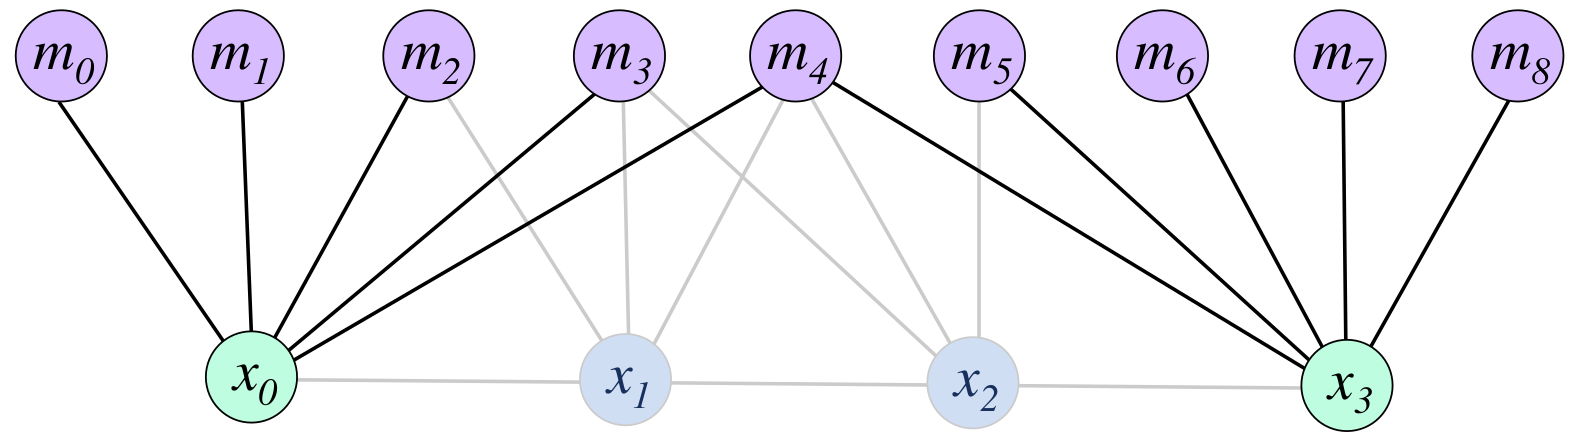
\includegraphics[width=0.75\textwidth]{images/keyframes}
   \caption{Sketch of the \ac{KF} principle}
   \label{fig:kf}
\end{figure}

In ORB-SLAM(2) \cite{Mur-Artal2015}, \cite{Mur-Artal2016}, on which this semester project is based, the following conditions must be fulfilled to insert a new \ac{KF}:

\begin{itemize}
  \item More than 20 frames must have passed from the last global relocalization
  \item Local mapping is idle, or more than 20 frames have passed from last \ac{KF} insertion
  \item Current frame tracks at least 50 points
  \item Current frame tracks less than 90\% points than the reference \ac{KF}
\end{itemize}

\subsubsection{\acf{KFM}}
A \acf{KFM} is if two \acp{KF}, one per client, observed the same location (cf. \autoref{fig:kfm1}). If a \ac{KFM} was detected, a transformation $T \in \text{Sim(3)}$ can be obtained from the poses of the \acp{KF}, which relates the maps of the two clients to each other (cf. \autoref{fig:kfm2}). With the transformation $T$ the maps than can be aligned (cf. \autoref{fig:kfm3}).

\begin{figure}[H]
  \centering
  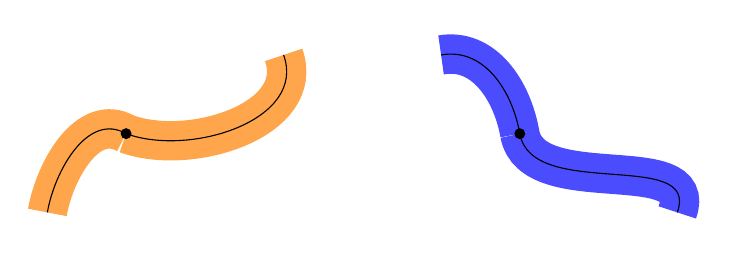
\begin{tikzpicture}
    \coordinate (A) at (0, 0);
    \coordinate (B) at (3, 2);
    \coordinate (C) at (5, 2);
    \coordinate (D1) at (1, 1);
    \coordinate (D2) at (6, 1);
    \coordinate (E) at (8, 0);

    \coordinate (F) at (0.9, 0.9);
    \coordinate (G) at (0.8, 1.1);
    \coordinate (H) at (1.1, 1.1);

    \node at (A) {};
    \node at (B) {};
    \node at (C) {};
    \node at (E) {};

    \draw [orange!70, line width=0.5cm] (A) to [out=80, in=150] (D1);
    \draw [orange!70, line width=0.5cm] (D1) to [out=-20, in=-70] (B);
    \draw [blue!70, line width=0.5cm] (C) to [out=10, in=100] (D2);
    \draw [blue!70, line width=0.5cm] (D2) to [out=-80, in=70] (E);
    \draw [black] (A) to [out=80, in=150] (D1);
    \draw [black] (D1) to [out=-20, in=-70] (B);
    \draw [black] (C) to [out=10, in=100] (D2);
    \draw [black] (D2) to [out=-80, in=70] (E);

    \node [fill=black, circle,inner sep=1pt, text width=0.5mm] at (D1) {};
    \node [fill=black, circle,inner sep=1pt, text width=0.5mm] at (D2) {};
  \end{tikzpicture}
  \caption{Two clients, each with own landmarks and \acp{KF} with one \ac{KF} observing the same location}
  \label{fig:kfm1}
\end{figure}

\begin{figure}[H]
  \centering
  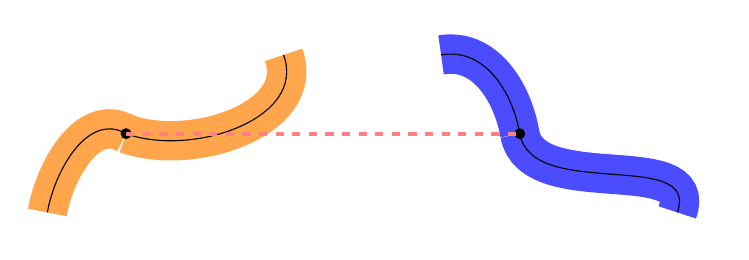
\begin{tikzpicture}
    \coordinate (A) at (0, 0);
    \coordinate (B) at (3, 2);
    \coordinate (C) at (5, 2);
    \coordinate (D1) at (1, 1);
    \coordinate (D2) at (6, 1);
    \coordinate (E) at (8, 0);

    \coordinate (F) at (0.9, 0.9);
    \coordinate (G) at (0.8, 1.1);
    \coordinate (H) at (1.1, 1.1);

    \node at (A) {};
    \node at (B) {};
    \node at (C) {};
    \node at (E) {};

    \draw [orange!70, line width=0.5cm] (A) to [out=80, in=150] (D1);
    \draw [orange!70, line width=0.5cm] (D1) to [out=-20, in=-70] (B);
    \draw [blue!70, line width=0.5cm] (C) to [out=10, in=100] (D2);
    \draw [blue!70, line width=0.5cm] (D2) to [out=-80, in=70] (E);
    \draw [black] (A) to [out=80, in=150] (D1);
    \draw [black] (D1) to [out=-20, in=-70] (B);
    \draw [black] (C) to [out=10, in=100] (D2);
    \draw [black] (D2) to [out=-80, in=70] (E);

    \node [fill=black, circle,inner sep=1pt, text width=0.5mm] at (D1) {};
    \node [fill=black, circle,inner sep=1pt, text width=0.5mm] at (D2) {};

    \draw [red!50, line width=0.05cm, dashed] (D1) to (D2);
  \end{tikzpicture}
  \caption{Transformation $T$ obtained from the poses of the two \acp{KF}}
  \label{fig:kfm2}
\end{figure}

\begin{figure}[H]
  \centering
  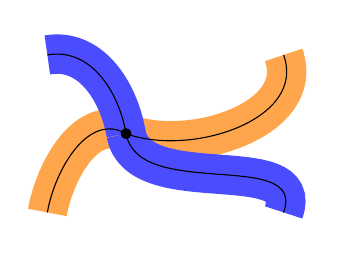
\begin{tikzpicture}
    \coordinate (A) at (0, 0);
    \coordinate (B) at (3, 2);
    \coordinate (C) at (0, 2);
    \coordinate (D) at (1, 1);
    \coordinate (E) at (3, 0);

    \coordinate (F) at (0.9, 0.9);
    \coordinate (G) at (0.8, 1.1);
    \coordinate (H) at (1.1, 1.1);

    \node at (A) {};
    \node at (B) {};
    \node at (C) {};
    \node at (E) {};

    \draw [orange!70, line width=0.5cm] (A) to [out=80, in=150] (D);
    \draw [orange!70, line width=0.5cm] (D) to [out=-20, in=-70] (B);
    \draw [blue!70, line width=0.5cm] (C) to [out=10, in=100] (D);
    \draw [blue!70, line width=0.5cm] (D) to [out=-80, in=70] (E);
    \draw [black] (A) to [out=80, in=150] (D);
    \draw [black] (D) to [out=-20, in=-70] (B);
    \draw [black] (C) to [out=10, in=100] (D);
    \draw [black] (D) to [out=-80, in=70] (E);

    \node [fill=black, circle,inner sep=1pt, text width=0.5mm] at (D) {};
  \end{tikzpicture}
  \caption{The two maps aligned}
  \label{fig:kfm3}
\end{figure}

In conclusion, a \ac{KFM} contains:
\begin{itemize}
  \item Two \acp{KF} (One per map/client)
  \item The transformation ($T \in \text{Sim(3)}$) between the two \acp{KF}
\end{itemize}

\subsubsection{Co-visibility graph}
Co-visibility is represented as an undirected, weighted graph, a co-visibility graph. Each node/vertex is a \ac{KF} and an edge between two \acp{KF} exists if they share observations of the same \acp{MP}. The weight of an edge is the number of common \acp{MP} \cite{Mur-Artal2015}. An example of \acp{KF} and the resulting co-visibility graph is shown in \autoref{fig:covis}.

\begin{figure}[H]
	\centering
	\subcaptionbox{\acp{KF} (blue), Current Camera (gree), \acp{MP} (black, red), Current Local \acp{MP} (red)\label{fig:covis1}}{\includegraphics[width=0.45\textwidth]{images/002.eps}}
	\quad
	\subcaptionbox{Co-visibility Graph\label{fig:covis2}}{\includegraphics[width=0.45\textwidth]{images/004.eps}}
	\caption{\acp{KF} and resulting co-visibility graph (Figures taken from \cite{Mur-Artal2015})}
	\label{fig:covis}
\end{figure}

\subsection{Previous approach}
In the previous approach, proposed in \cite{Schmuck2017}, as soon as a \ac{KFM} was detected, the maps were fused. In a real world example this procedure looks the following:

\begin{enumerate}
  \item {Two clients observed the same location (shown in figure \autoref{fig:kfm4})
    \begin{figure}[H]
      \centering
      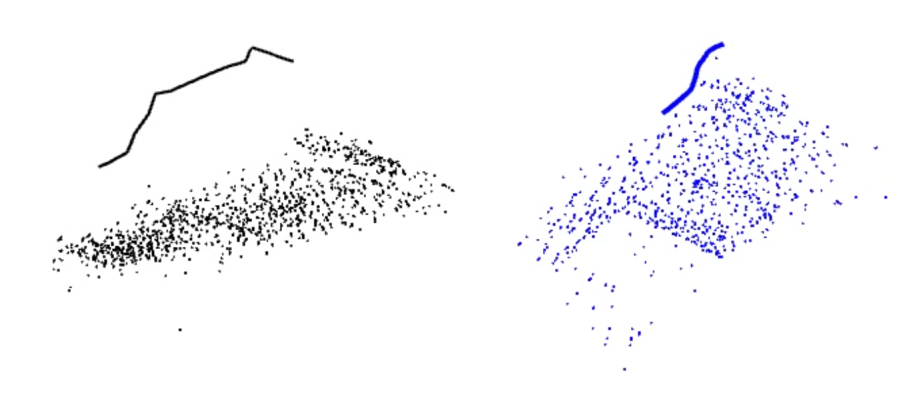
\includegraphics[width=0.75\textwidth]{images/map_1_2_1}
      \caption{Two clients, each with own landmarks and \acp{KF} observing the same location}
      \label{fig:kfm4}
    \end{figure}}
  \item {The transformation between the two maps can be obtained (shown in figure \autoref{fig:kfm5})
    \begin{figure}[H]
      \centering
      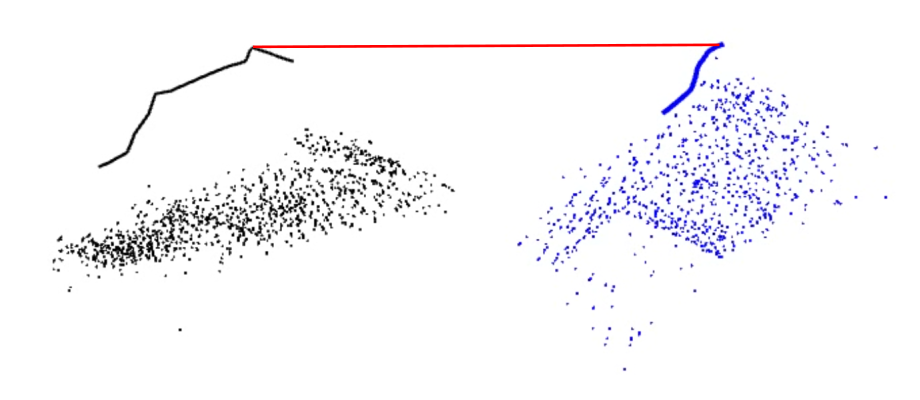
\includegraphics[width=0.75\textwidth]{images/map_1_2_2}
      \caption{Transformation $T$ obtained from the poses of the two \acp{KF}}
      \label{fig:kfm5}
    \end{figure}}
  \item {The maps can be aligned (shown in figure \autoref{fig:kfm6})
    \begin{figure}[H]
      \centering
      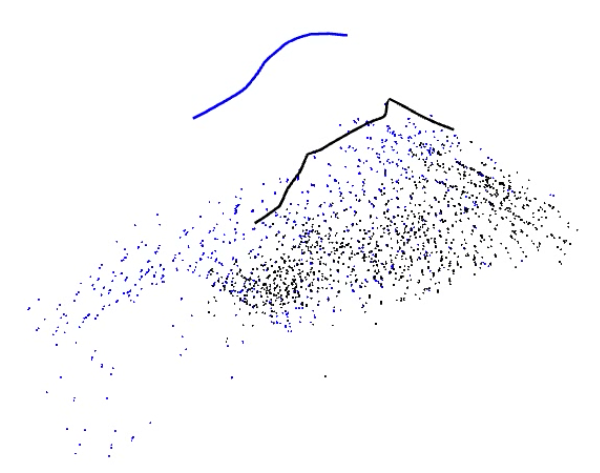
\includegraphics[width=0.75\textwidth]{images/map_1_2_merge}
      \caption{Aligned maps}
      \label{fig:kfm6}
    \end{figure}}
  \item Perform \acf{PGO}
  \item Perform \acf{BA}
\end{enumerate}

\subsection{Proposed approach}
The general idea of the proposed approach is to use multiple \acp{KFM} to guarantee no false map alignment, to reduce drift and to achieve higher accuracy. If maps are only fused when multiple \acp{KFM} were detected, one false \ac{KFM} won't result in a wrong aligned fused map, which could happened with the previous approach. The usage of multiple \acp{KFM} provides the \ac{PGO} and the \ac{BA} with more information which should lead to a reduced drift and a higher accuracy.\\

The proposed map fusion approach works as follow:

\begin{enumerate}
  \item After a \ac{KFM} is found, skip $m$ \acp{KF} before processing the next \acs{KF}
  \item Wait until $n$ \acp{KFM} were detected
  \item Fuse the two maps with the transformation of one of the \acp{KFM}
  \item Fuse the map points in the ($n-1$) \acp{KFM}
  \item Perform \ac{PGO}
  \item Perform \ac{BA}
\end{enumerate}

To give the reader a better intuition about how the proposed map fusion approach works, it will be visualized in a synthetic example step by step.\\
The example starts with two \acp{KF}, one per client, which are checked if they observe the same location (cf. \autoref{fig:newapproach1}). If a \ac{KFM} was detected, as in \autoref{fig:newapproach2}, $m$, in this example five, \acp{KF} are skipped before processing the next \acp{KF}.

\begin{figure}[H]
    \centering
    \subcaptionbox{Two client with one \ac{KF}\label{fig:newapproach1}}{
      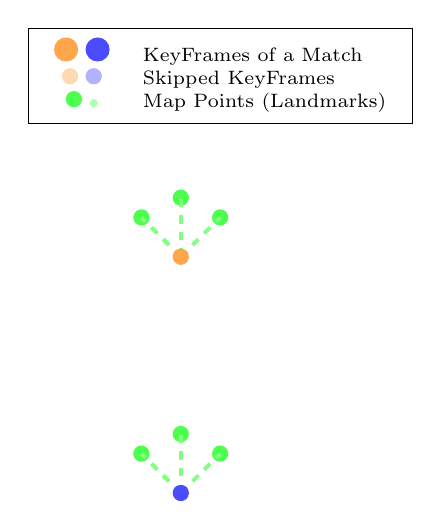
\begin{tikzpicture}
        \coordinate (A1) at (0, 3);
        \coordinate (A1MP1) at (-0.5, 3.5);
        \coordinate (A1MP2) at (0, 3.75);
        \coordinate (A1MP3) at (0.5, 3.5);

        \coordinate (A2) at (0, 0);
        \coordinate (A2MP1) at (-0.5, 0.5);
        \coordinate (A2MP2) at (0, 0.75);
        \coordinate (A2MP3) at (0.5, 0.5);

        \node [fill=green!70, circle,inner sep=2pt, text width=0.1mm] at (A1MP1) {};
        \node [fill=green!70, circle,inner sep=2pt, text width=0.1mm] at (A1MP2) {};
        \node [fill=green!70, circle,inner sep=2pt, text width=0.1mm] at (A1MP3) {};
        \draw [green!50, dashed, line width=0.05cm] (A1) to (A1MP1);
        \draw [green!50, dashed, line width=0.05cm] (A1) to (A1MP2);
        \draw [green!50, dashed, line width=0.05cm] (A1) to (A1MP3);
        \node [fill=orange!70, circle,inner sep=2pt, text width=0.1mm] at (A1) {};

        \node [fill=green!70, circle,inner sep=2pt, text width=0.1mm] at (A2MP1) {};
        \node [fill=green!70, circle,inner sep=2pt, text width=0.1mm] at (A2MP2) {};
        \node [fill=green!70, circle,inner sep=2pt, text width=0.1mm] at (A2MP3) {}; \draw [green!50, dashed, line width=0.05cm] (A2) to (A2MP1);
        \draw [green!50, dashed, line width=0.05cm] (A2) to (A2MP2);
        \draw [green!50, dashed, line width=0.05cm] (A2) to (A2MP3);
        \node [fill=blue!70, circle,inner sep=2pt, text width=0.1mm] at (A2) {};

        \node[draw] at (0.5, 5.3)
        {
          \scriptsize
          \begin{tabular}{cl}
            \tikz\node[fill=orange!70, circle,inner sep=3pt, text width=0.1mm] {}; \tikz\node[fill=blue!70, circle,inner sep=3pt, text width=0.1mm] {}; & KeyFrames of a Match \\
            \tikz\node[fill=orange!30, circle,inner sep=2pt, text width=0.1mm] {}; \tikz\node[fill=blue!30, circle,inner sep=2pt, text width=0.1mm] {}; & Skipped KeyFrames \\
            \tikz\node [fill=green!70, circle, inner sep=2pt, text width=0.1mm] {}; \tikz\node[fill=green!30, circle,inner sep=1pt, text width=0.1mm] {}; & Map Points (Landmarks)
          \end{tabular}
        };
      \end{tikzpicture}}%}
      \quad
    \subcaptionbox{First \ac{KFM}\label{fig:newapproach2}}{
      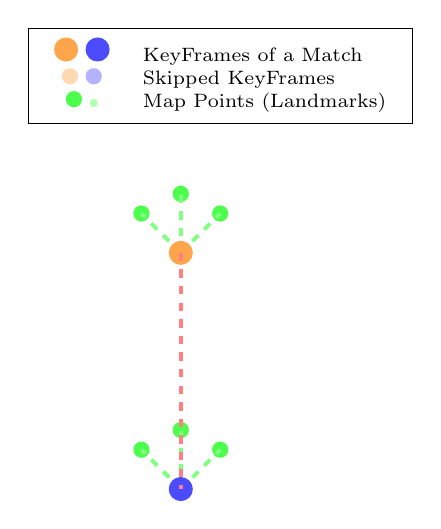
\begin{tikzpicture}
        \coordinate (A1) at (0, 3);
        \coordinate (A1MP1) at (-0.5, 3.5);
        \coordinate (A1MP2) at (0, 3.75);
        \coordinate (A1MP3) at (0.5, 3.5);

        \coordinate (A2) at (0, 0);
        \coordinate (A2MP1) at (-0.5, 0.5);
        \coordinate (A2MP2) at (0, 0.75);
        \coordinate (A2MP3) at (0.5, 0.5);

        \node [fill=green!70, circle,inner sep=2pt, text width=0.1mm] at (A1MP1) {};
        \node [fill=green!70, circle,inner sep=2pt, text width=0.1mm] at (A1MP2) {};
        \node [fill=green!70, circle,inner sep=2pt, text width=0.1mm] at (A1MP3) {};
        \draw [green!50, dashed, line width=0.05cm] (A1) to (A1MP1);
        \draw [green!50, dashed, line width=0.05cm] (A1) to (A1MP2);
        \draw [green!50, dashed, line width=0.05cm] (A1) to (A1MP3);
        \node [fill=orange!70, circle,inner sep=3pt, text width=0.1mm] at (A1) {};

        \node [fill=green!70, circle,inner sep=2pt, text width=0.1mm] at (A2MP1) {};
        \node [fill=green!70, circle,inner sep=2pt, text width=0.1mm] at (A2MP2) {};
        \node [fill=green!70, circle,inner sep=2pt, text width=0.1mm] at (A2MP3) {};
        \draw [green!50, dashed, line width=0.05cm] (A2) to (A2MP1);
        \draw [green!50, dashed, line width=0.05cm] (A2) to (A2MP2);
        \draw [green!50, dashed, line width=0.05cm] (A2) to (A2MP3);
        \node [fill=blue!70, circle,inner sep=3pt, text width=0.1mm] at (A2) {};

        \draw [red!50, line width=0.05cm, dashed] (A1) to (A2);

        \node[draw] at (0.5, 5.25)
        {
          \scriptsize
          \begin{tabular}{cl}
            \tikz\node[fill=orange!70, circle,inner sep=3pt, text width=0.1mm] {}; \tikz\node[fill=blue!70, circle,inner sep=3pt, text width=0.1mm] {}; & KeyFrames of a Match \\
            \tikz\node[fill=orange!30, circle,inner sep=2pt, text width=0.1mm] {}; \tikz\node[fill=blue!30, circle,inner sep=2pt, text width=0.1mm] {}; & Skipped KeyFrames \\
            \tikz\node [fill=green!70, circle, inner sep=2pt, text width=0.1mm] {}; \tikz\node[fill=green!30, circle,inner sep=1pt, text width=0.1mm] {}; & Map Points (Landmarks)
          \end{tabular}
        };
      \end{tikzpicture}}
      \caption{First two steps of the map fusion example}
      \label{fig:newapproach12}
\end{figure}


\begin{figure}[H]
  \centering
  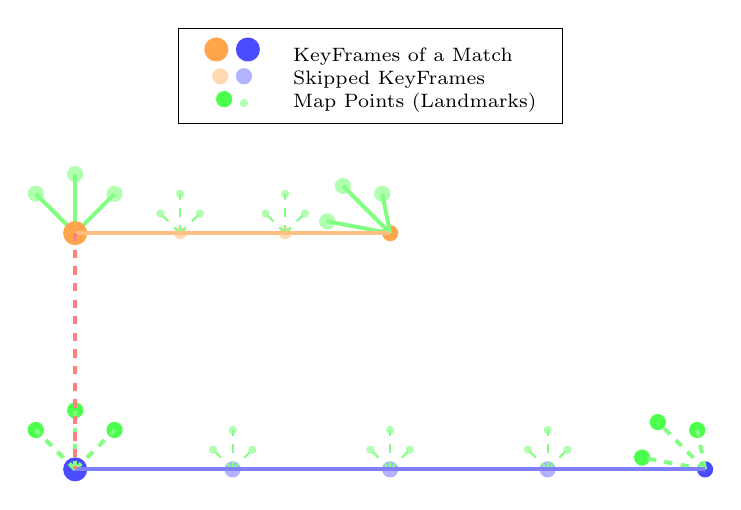
\begin{tikzpicture}
    \coordinate (A1) at (0, 3);
    \coordinate (A1MP1) at (-0.5, 3.5);
    \coordinate (A1MP2) at (0, 3.75);
    \coordinate (A1MP3) at (0.5, 3.5);

    \coordinate (AB11) at (4/3, 3);
    \coordinate (AB11MP1) at (-0.25+4/3, 3.25);
    \coordinate (AB11MP2) at (4/3, 3.5);
    \coordinate (AB11MP3) at (0.25+4/3, 3.25);

    \coordinate (AB12) at (8/3, 3);
    \coordinate (AB12MP1) at (-0.25+8/3, 3.25);
    \coordinate (AB12MP2) at (8/3, 3.5);
    \coordinate (AB12MP3) at (0.25+8/3, 3.25);

    \coordinate (B1) at (4, 3);
    \coordinate (B1MP1) at (3.2, 3.15);
    \coordinate (B1MP2) at (3.4, 3.6);
    \coordinate (B1MP3) at (3.9, 3.5);

    \coordinate (A2) at (0, 0);
    \coordinate (A2MP1) at (-0.5, 0.5);
    \coordinate (A2MP2) at (0, 0.75);
    \coordinate (A2MP3) at (0.5, 0.5);

    \coordinate (AB21) at (2, 0);
    \coordinate (AB21MP1) at (1.75, 0.25);
    \coordinate (AB21MP2) at (2, 0.5);
    \coordinate (AB21MP3) at (2.25, 0.25);

    \coordinate (AB22) at (4, 0);
    \coordinate (AB22MP1) at (3.75, 0.25);
    \coordinate (AB22MP2) at (4, 0.5);
    \coordinate (AB22MP3) at (4.25, 0.25);

    \coordinate (AB23) at (6, 0);
    \coordinate (AB23MP1) at (5.75, 0.25);
    \coordinate (AB23MP2) at (6, 0.5);
    \coordinate (AB23MP3) at (6.25, 0.25);

    \coordinate (B2) at (8, 0);
    \coordinate (B2MP1) at (7.2, 0.15);
    \coordinate (B2MP2) at (7.4, 0.6);
    \coordinate (B2MP3) at (7.9, 0.5);


    \node [fill=green!30, circle,inner sep=2pt, text width=0.1mm] at (A1MP1) {};
    \node [fill=green!30, circle,inner sep=2pt, text width=0.1mm] at (A1MP2) {};
    \node [fill=green!30, circle,inner sep=2pt, text width=0.1mm] at (A1MP3) {};
    \draw [green!50, line width=0.05cm] (A1) to (A1MP1);
    \draw [green!50, line width=0.05cm] (A1) to (A1MP2);
    \draw [green!50, line width=0.05cm] (A1) to (A1MP3);
    \node [fill=orange!70, circle,inner sep=3pt, text width=0.1mm] at (A1) {};

    \node [fill=orange!30, circle,inner sep=1.5pt, text width=0.1mm] at (AB11) {};
    \node [fill=green!30, circle,inner sep=1pt, text width=0.1mm] at (AB11MP1) {};
    \node [fill=green!30, circle,inner sep=1pt, text width=0.1mm] at (AB11MP2) {};
    \node [fill=green!30, circle,inner sep=1pt, text width=0.1mm] at (AB11MP3) {};
    \draw [green!50, dashed, line width=0.025cm] (AB11) to (AB11MP1);
    \draw [green!50, dashed, line width=0.025cm] (AB11) to (AB11MP2);
    \draw [green!50, dashed, line width=0.025cm] (AB11) to (AB11MP3);

    \node [fill=orange!30, circle,inner sep=1.5pt, text width=0.1mm] at (AB12) {};
    \node [fill=green!30, circle,inner sep=1pt, text width=0.1mm] at (AB12MP1) {};
    \node [fill=green!30, circle,inner sep=1pt, text width=0.1mm] at (AB12MP2) {};
    \node [fill=green!30, circle,inner sep=1pt, text width=0.1mm] at (AB12MP3) {};
    \draw [green!50, dashed, line width=0.025cm] (AB12) to (AB12MP1);
    \draw [green!50, dashed, line width=0.025cm] (AB12) to (AB12MP2);
    \draw [green!50, dashed, line width=0.025cm] (AB12) to (AB12MP3);

    \node [fill=orange!70, circle,inner sep=2pt, text width=0.1mm] at (B1) {};
    \node [fill=green!30, circle, inner sep=2pt, text width=0.1mm] at (B1MP1) {};
    \node [fill=green!30, circle, inner sep=2pt, text width=0.1mm] at (B1MP2) {};
    \node [fill=green!30, circle, inner sep=2pt, text width=0.1mm] at (B1MP3) {};
    \draw [green!50, line width=0.05cm] (B1) to (B1MP1);
    \draw [green!50, line width=0.05cm] (B1) to (B1MP2);
    \draw [green!50, line width=0.05cm] (B1) to (B1MP3);

    \node [fill=blue!70, circle,inner sep=3pt, text width=0.1mm] at (A2) {};
    \node [fill=green!70, circle,inner sep=2pt, text width=0.1mm] at (A2MP1) {};
    \node [fill=green!70, circle,inner sep=2pt, text width=0.1mm] at (A2MP2) {};
    \node [fill=green!70, circle,inner sep=2pt, text width=0.1mm] at (A2MP3) {};
    \draw [green!50, dashed, line width=0.05cm] (A2) to (A2MP1);
    \draw [green!50, dashed, line width=0.05cm] (A2) to (A2MP2);
    \draw [green!50, dashed, line width=0.05cm] (A2) to (A2MP3);

    \node [fill=blue!30, circle,inner sep=2pt, text width=0.1mm] at (AB21) {};
    \node [fill=green!30, circle,inner sep=1pt, text width=0.1mm] at (AB21MP1) {};
    \node [fill=green!30, circle,inner sep=1pt, text width=0.1mm] at (AB21MP2) {};
    \node [fill=green!30, circle,inner sep=1pt, text width=0.1mm] at (AB21MP3) {};
    \draw [green!50, dashed, line width=0.025cm] (AB21) to (AB21MP1);
    \draw [green!50, dashed, line width=0.025cm] (AB21) to (AB21MP2);
    \draw [green!50, dashed, line width=0.025cm] (AB21) to (AB21MP3);

    \node [fill=blue!30, circle,inner sep=2pt, text width=0.1mm] at (AB22) {};
    \node [fill=green!30, circle,inner sep=1pt, text width=0.1mm] at (AB22MP1) {};
    \node [fill=green!30, circle,inner sep=1pt, text width=0.1mm] at (AB22MP2) {};
    \node [fill=green!30, circle,inner sep=1pt, text width=0.1mm] at (AB22MP3) {};
    \draw [green!50, dashed, line width=0.025cm] (AB22) to (AB22MP1);
    \draw [green!50, dashed, line width=0.025cm] (AB22) to (AB22MP2);
    \draw [green!50, dashed, line width=0.025cm] (AB22) to (AB22MP3);

    \node [fill=blue!30, circle,inner sep=2pt, text width=0.1mm] at (AB23) {};
    \node [fill=green!30, circle,inner sep=1pt, text width=0.1mm] at (AB23MP1) {};
    \node [fill=green!30, circle,inner sep=1pt, text width=0.1mm] at (AB23MP2) {};
    \node [fill=green!30, circle,inner sep=1pt, text width=0.1mm] at (AB23MP3) {};
    \draw [green!50, dashed, line width=0.025cm] (AB23) to (AB23MP1);
    \draw [green!50, dashed, line width=0.025cm] (AB23) to (AB23MP2);
    \draw [green!50, dashed, line width=0.025cm] (AB23) to (AB23MP3);

    \node [fill=blue!70, circle,inner sep=2pt, text width=0.1mm] at (B2) {};
    \node [fill=green!70, circle,inner sep=2pt, text width=0.1mm] at (B2MP1) {};
    \node [fill=green!70, circle,inner sep=2pt, text width=0.1mm] at (B2MP2) {};
    \node [fill=green!70, circle,inner sep=2pt, text width=0.1mm] at (B2MP3) {};
    \draw [green!50, dashed, line width=0.05cm] (B2) to (B2MP1);
    \draw [green!50, dashed, line width=0.05cm] (B2) to (B2MP2);
    \draw [green!50, dashed, line width=0.05cm] (B2) to (B2MP3);

    \draw [orange!50, line width=0.05cm] (A1) to (B1);
    \draw [blue!50, line width=0.05cm] (A2) to (B2);

    \draw [red!50, line width=0.05cm, dashed] (A1) to (A2);

    \node[draw] at (3.75, 5.0)
    {
      \scriptsize
      \begin{tabular}{cl}
        \tikz\node[fill=orange!70, circle,inner sep=3pt, text width=0.1mm] {}; \tikz\node[fill=blue!70, circle,inner sep=3pt, text width=0.1mm] {}; & KeyFrames of a Match \\
        \tikz\node[fill=orange!30, circle,inner sep=2pt, text width=0.1mm] {}; \tikz\node[fill=blue!30, circle,inner sep=2pt, text width=0.1mm] {}; & Skipped KeyFrames \\
        \tikz\node [fill=green!70, circle, inner sep=2pt, text width=0.1mm] {}; \tikz\node[fill=green!30, circle,inner sep=1pt, text width=0.1mm] {}; & Map Points (Landmarks)
      \end{tabular}
    };
  \end{tikzpicture}
  \caption{Skipped five \acp{KF}}
  \label{fig:newapproach3}
\end{figure}

After $m(= 5)$ \acp{KF} are skipped, the system checks again, if a \ac{KFM} can be detected, shown in \autoref{fig:newapproach3}. \autoref{fig:newapproach4} then shows the case, where the next \ac{KFM} was detected.

\begin{figure}[H]
  \centering
  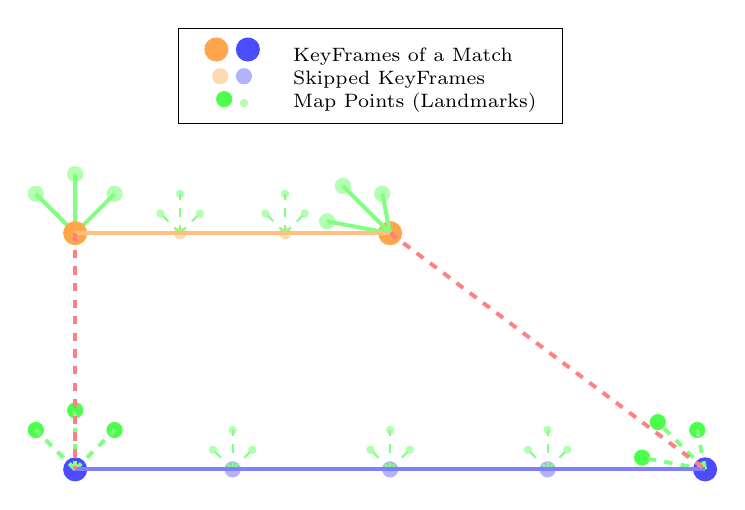
\begin{tikzpicture}
    \coordinate (A1) at (0, 3);
    \coordinate (A1MP1) at (-0.5, 3.5);
    \coordinate (A1MP2) at (0, 3.75);
    \coordinate (A1MP3) at (0.5, 3.5);

    \coordinate (AB11) at (4/3, 3);
    \coordinate (AB11MP1) at (-0.25+4/3, 3.25);
    \coordinate (AB11MP2) at (4/3, 3.5);
    \coordinate (AB11MP3) at (0.25+4/3, 3.25);

    \coordinate (AB12) at (8/3, 3);
    \coordinate (AB12MP1) at (-0.25+8/3, 3.25);
    \coordinate (AB12MP2) at (8/3, 3.5);
    \coordinate (AB12MP3) at (0.25+8/3, 3.25);

    \coordinate (B1) at (4, 3);
    \coordinate (B1MP1) at (3.2, 3.15);
    \coordinate (B1MP2) at (3.4, 3.6);
    \coordinate (B1MP3) at (3.9, 3.5);

    \coordinate (A2) at (0, 0);
    \coordinate (A2MP1) at (-0.5, 0.5);
    \coordinate (A2MP2) at (0, 0.75);
    \coordinate (A2MP3) at (0.5, 0.5);

    \coordinate (AB21) at (2, 0);
    \coordinate (AB21MP1) at (1.75, 0.25);
    \coordinate (AB21MP2) at (2, 0.5);
    \coordinate (AB21MP3) at (2.25, 0.25);

    \coordinate (AB22) at (4, 0);
    \coordinate (AB22MP1) at (3.75, 0.25);
    \coordinate (AB22MP2) at (4, 0.5);
    \coordinate (AB22MP3) at (4.25, 0.25);

    \coordinate (AB23) at (6, 0);
    \coordinate (AB23MP1) at (5.75, 0.25);
    \coordinate (AB23MP2) at (6, 0.5);
    \coordinate (AB23MP3) at (6.25, 0.25);

    \coordinate (B2) at (8, 0);
    \coordinate (B2MP1) at (7.2, 0.15);
    \coordinate (B2MP2) at (7.4, 0.6);
    \coordinate (B2MP3) at (7.9, 0.5);


    \node [fill=green!30, circle,inner sep=2pt, text width=0.1mm] at (A1MP1) {};
    \node [fill=green!30, circle,inner sep=2pt, text width=0.1mm] at (A1MP2) {};
    \node [fill=green!30, circle,inner sep=2pt, text width=0.1mm] at (A1MP3) {};
    \draw [green!50, line width=0.05cm] (A1) to (A1MP1);
    \draw [green!50, line width=0.05cm] (A1) to (A1MP2);
    \draw [green!50, line width=0.05cm] (A1) to (A1MP3);
    \node [fill=orange!70, circle,inner sep=3pt, text width=0.1mm] at (A1) {};

    \node [fill=orange!30, circle,inner sep=1.5pt, text width=0.1mm] at (AB11) {};
    \node [fill=green!30, circle,inner sep=1pt, text width=0.1mm] at (AB11MP1) {};
    \node [fill=green!30, circle,inner sep=1pt, text width=0.1mm] at (AB11MP2) {};
    \node [fill=green!30, circle,inner sep=1pt, text width=0.1mm] at (AB11MP3) {};
    \draw [green!50, dashed, line width=0.025cm] (AB11) to (AB11MP1);
    \draw [green!50, dashed, line width=0.025cm] (AB11) to (AB11MP2);
    \draw [green!50, dashed, line width=0.025cm] (AB11) to (AB11MP3);

    \node [fill=orange!30, circle,inner sep=1.5pt, text width=0.1mm] at (AB12) {};
    \node [fill=green!30, circle,inner sep=1pt, text width=0.1mm] at (AB12MP1) {};
    \node [fill=green!30, circle,inner sep=1pt, text width=0.1mm] at (AB12MP2) {};
    \node [fill=green!30, circle,inner sep=1pt, text width=0.1mm] at (AB12MP3) {};
    \draw [green!50, dashed, line width=0.025cm] (AB12) to (AB12MP1);
    \draw [green!50, dashed, line width=0.025cm] (AB12) to (AB12MP2);
    \draw [green!50, dashed, line width=0.025cm] (AB12) to (AB12MP3);

    \node [fill=orange!70, circle,inner sep=3pt, text width=0.1mm] at (B1) {};
    \node [fill=green!30, circle, inner sep=2pt, text width=0.1mm] at (B1MP1) {};
    \node [fill=green!30, circle, inner sep=2pt, text width=0.1mm] at (B1MP2) {};
    \node [fill=green!30, circle, inner sep=2pt, text width=0.1mm] at (B1MP3) {};
    \draw [green!50, line width=0.05cm] (B1) to (B1MP1);
    \draw [green!50, line width=0.05cm] (B1) to (B1MP2);
    \draw [green!50, line width=0.05cm] (B1) to (B1MP3);

    \node [fill=blue!70, circle,inner sep=3pt, text width=0.1mm] at (A2) {};
    \node [fill=green!70, circle,inner sep=2pt, text width=0.1mm] at (A2MP1) {};
    \node [fill=green!70, circle,inner sep=2pt, text width=0.1mm] at (A2MP2) {};
    \node [fill=green!70, circle,inner sep=2pt, text width=0.1mm] at (A2MP3) {};
    \draw [green!50, dashed, line width=0.05cm] (A2) to (A2MP1);
    \draw [green!50, dashed, line width=0.05cm] (A2) to (A2MP2);
    \draw [green!50, dashed, line width=0.05cm] (A2) to (A2MP3);

    \node [fill=blue!30, circle,inner sep=2pt, text width=0.1mm] at (AB21) {};
    \node [fill=green!30, circle,inner sep=1pt, text width=0.1mm] at (AB21MP1) {};
    \node [fill=green!30, circle,inner sep=1pt, text width=0.1mm] at (AB21MP2) {};
    \node [fill=green!30, circle,inner sep=1pt, text width=0.1mm] at (AB21MP3) {};
    \draw [green!50, dashed, line width=0.025cm] (AB21) to (AB21MP1);
    \draw [green!50, dashed, line width=0.025cm] (AB21) to (AB21MP2);
    \draw [green!50, dashed, line width=0.025cm] (AB21) to (AB21MP3);

    \node [fill=blue!30, circle,inner sep=2pt, text width=0.1mm] at (AB22) {};
    \node [fill=green!30, circle,inner sep=1pt, text width=0.1mm] at (AB22MP1) {};
    \node [fill=green!30, circle,inner sep=1pt, text width=0.1mm] at (AB22MP2) {};
    \node [fill=green!30, circle,inner sep=1pt, text width=0.1mm] at (AB22MP3) {};
    \draw [green!50, dashed, line width=0.025cm] (AB22) to (AB22MP1);
    \draw [green!50, dashed, line width=0.025cm] (AB22) to (AB22MP2);
    \draw [green!50, dashed, line width=0.025cm] (AB22) to (AB22MP3);

    \node [fill=blue!30, circle,inner sep=2pt, text width=0.1mm] at (AB23) {};
    \node [fill=green!30, circle,inner sep=1pt, text width=0.1mm] at (AB23MP1) {};
    \node [fill=green!30, circle,inner sep=1pt, text width=0.1mm] at (AB23MP2) {};
    \node [fill=green!30, circle,inner sep=1pt, text width=0.1mm] at (AB23MP3) {};
    \draw [green!50, dashed, line width=0.025cm] (AB23) to (AB23MP1);
    \draw [green!50, dashed, line width=0.025cm] (AB23) to (AB23MP2);
    \draw [green!50, dashed, line width=0.025cm] (AB23) to (AB23MP3);

    \node [fill=blue!70, circle,inner sep=3pt, text width=0.1mm] at (B2) {};
    \node [fill=green!70, circle,inner sep=2pt, text width=0.1mm] at (B2MP1) {};
    \node [fill=green!70, circle,inner sep=2pt, text width=0.1mm] at (B2MP2) {};
    \node [fill=green!70, circle,inner sep=2pt, text width=0.1mm] at (B2MP3) {};
    \draw [green!50, dashed, line width=0.05cm] (B2) to (B2MP1);
    \draw [green!50, dashed, line width=0.05cm] (B2) to (B2MP2);
    \draw [green!50, dashed, line width=0.05cm] (B2) to (B2MP3);

    \draw [orange!50, line width=0.05cm] (A1) to (B1);
    \draw [blue!50, line width=0.05cm] (A2) to (B2);

    \draw [red!50, line width=0.05cm, dashed] (A1) to (A2);
    \draw [red!50, line width=0.05cm, dashed] (B1) to (B2);

    \node[draw] at (3.75, 5.0)
    {
      \scriptsize
      \begin{tabular}{cl}
        \tikz\node[fill=orange!70, circle,inner sep=3pt, text width=0.1mm] {}; \tikz\node[fill=blue!70, circle,inner sep=3pt, text width=0.1mm] {}; & KeyFrames of a Match \\
        \tikz\node[fill=orange!30, circle,inner sep=2pt, text width=0.1mm] {}; \tikz\node[fill=blue!30, circle,inner sep=2pt, text width=0.1mm] {}; & Skipped KeyFrames \\
        \tikz\node [fill=green!70, circle, inner sep=2pt, text width=0.1mm] {}; \tikz\node[fill=green!30, circle,inner sep=1pt, text width=0.1mm] {}; & Map Points (Landmarks)
      \end{tabular}
    };
  \end{tikzpicture}
  \caption{Next \acp{KF}}
  \label{fig:newapproach4}
\end{figure}

\begin{figure}[H]
  \centering
  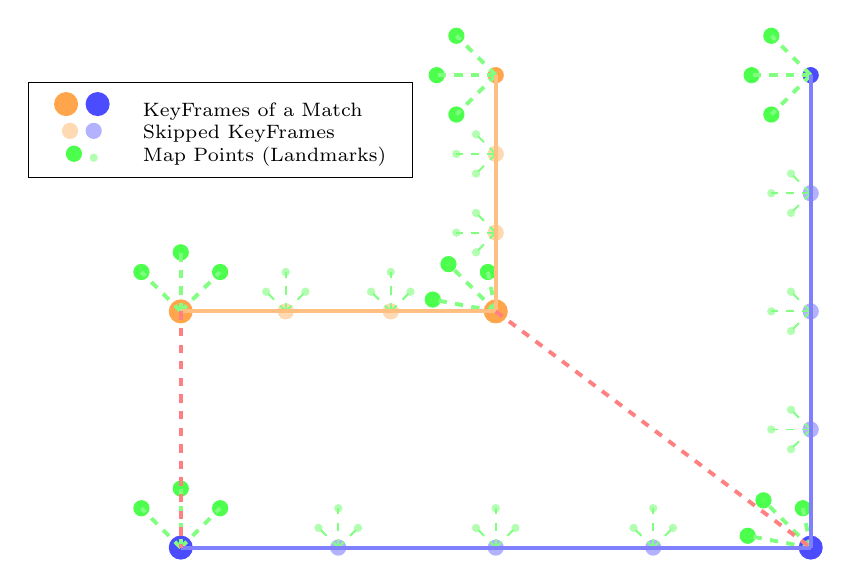
\begin{tikzpicture}
    \coordinate (A1) at (0, 3);
    \coordinate (A1MP1) at (-0.5, 3.5);
    \coordinate (A1MP2) at (0, 3.75);
    \coordinate (A1MP3) at (0.5, 3.5);

    \coordinate (AB11) at (4/3, 3);
    \coordinate (AB11MP1) at (-0.25+4/3, 3.25);
    \coordinate (AB11MP2) at (4/3, 3.5);
    \coordinate (AB11MP3) at (0.25+4/3, 3.25);

    \coordinate (AB12) at (8/3, 3);
    \coordinate (AB12MP1) at (-0.25+8/3, 3.25);
    \coordinate (AB12MP2) at (8/3, 3.5);
    \coordinate (AB12MP3) at (0.25+8/3, 3.25);

    \coordinate (B1) at (4, 3);
    \coordinate (B1MP1) at (3.2, 3.15);
    \coordinate (B1MP2) at (3.4, 3.6);
    \coordinate (B1MP3) at (3.9, 3.5);

    \coordinate (BC11) at (4, 4);
    \coordinate (BC11MP1) at (3.75, 4.25);
    \coordinate (BC11MP2) at (3.5, 4.0);
    \coordinate (BC11MP3) at (3.75, 3.75);

    \coordinate (BC12) at (4, 5);
    \coordinate (BC12MP1) at (3.75, 5.25);
    \coordinate (BC12MP2) at (3.5, 5.0);
    \coordinate (BC12MP3) at (3.75, 4.75);

    \coordinate (C1) at (4, 6);
    \coordinate (C1MP1) at (3.5, 6.5);
    \coordinate (C1MP2) at (3.25, 6.0);
    \coordinate (C1MP3) at (3.5, 5.5);

    \coordinate (A2) at (0, 0);
    \coordinate (A2MP1) at (-0.5, 0.5);
    \coordinate (A2MP2) at (0, 0.75);
    \coordinate (A2MP3) at (0.5, 0.5);

    \coordinate (AB21) at (2, 0);
    \coordinate (AB21MP1) at (1.75, 0.25);
    \coordinate (AB21MP2) at (2, 0.5);
    \coordinate (AB21MP3) at (2.25, 0.25);

    \coordinate (AB22) at (4, 0);
    \coordinate (AB22MP1) at (3.75, 0.25);
    \coordinate (AB22MP2) at (4, 0.5);
    \coordinate (AB22MP3) at (4.25, 0.25);

    \coordinate (AB23) at (6, 0);
    \coordinate (AB23MP1) at (5.75, 0.25);
    \coordinate (AB23MP2) at (6, 0.5);
    \coordinate (AB23MP3) at (6.25, 0.25);

    \coordinate (B2) at (8, 0);
    \coordinate (B2MP1) at (7.2, 0.15);
    \coordinate (B2MP2) at (7.4, 0.6);
    \coordinate (B2MP3) at (7.9, 0.5);

    \coordinate (BC21) at (8, 1.5);
    \coordinate (BC21MP1) at (7.75, 1.75);
    \coordinate (BC21MP2) at (7.5, 1.5);
    \coordinate (BC21MP3) at (7.75, 1.25);

    \coordinate (BC22) at (8, 3);
    \coordinate (BC22MP1) at (7.75, 3.25);
    \coordinate (BC22MP2) at (7.5, 3.0);
    \coordinate (BC22MP3) at (7.75, 2.75);

    \coordinate (BC23) at (8, 4.5);
    \coordinate (BC23MP1) at (7.75, 4.75);
    \coordinate (BC23MP2) at (7.5, 4.5);
    \coordinate (BC23MP3) at (7.75, 4.25);

    \coordinate (C2) at (8, 6);
    \coordinate (C2MP1) at (7.5, 6.5);
    \coordinate (C2MP2) at (7.25, 6.0);
    \coordinate (C2MP3) at (7.5, 5.5);

    \node [fill=orange!70, circle,inner sep=3pt, text width=0.1mm] at (A1) {};
    \node [fill=green!70, circle,inner sep=2pt, text width=0.1mm] at (A1MP1) {};
    \node [fill=green!70, circle,inner sep=2pt, text width=0.1mm] at (A1MP2) {};
    \node [fill=green!70, circle,inner sep=2pt, text width=0.1mm] at (A1MP3) {};
    \draw [green!50, dashed, line width=0.05cm] (A1) to (A1MP1);
    \draw [green!50, dashed, line width=0.05cm] (A1) to (A1MP2);
    \draw [green!50, dashed, line width=0.05cm] (A1) to (A1MP3);

    \node [fill=orange!30, circle,inner sep=2pt, text width=0.1mm] at (AB11) {};
    \node [fill=green!30, circle,inner sep=1pt, text width=0.1mm] at (AB11MP1) {};
    \node [fill=green!30, circle,inner sep=1pt, text width=0.1mm] at (AB11MP2) {};
    \node [fill=green!30, circle,inner sep=1pt, text width=0.1mm] at (AB11MP3) {};
    \draw [green!50, dashed, line width=0.025cm] (AB11) to (AB11MP1);
    \draw [green!50, dashed, line width=0.025cm] (AB11) to (AB11MP2);
    \draw [green!50, dashed, line width=0.025cm] (AB11) to (AB11MP3);

    \node [fill=orange!30, circle,inner sep=2pt, text width=0.1mm] at (AB12) {};
    \node [fill=green!30, circle,inner sep=1pt, text width=0.1mm] at (AB12MP1) {};
    \node [fill=green!30, circle,inner sep=1pt, text width=0.1mm] at (AB12MP2) {};
    \node [fill=green!30, circle,inner sep=1pt, text width=0.1mm] at (AB12MP3) {};
    \draw [green!50, dashed, line width=0.025cm] (AB12) to (AB12MP1);
    \draw [green!50, dashed, line width=0.025cm] (AB12) to (AB12MP2);
    \draw [green!50, dashed, line width=0.025cm] (AB12) to (AB12MP3);

    \node [fill=orange!70, circle, inner sep=3pt, text width=0.1mm] at (B1) {};
    \node [fill=green!70, circle, inner sep=2pt, text width=0.1mm] at (B1MP1) {};
    \node [fill=green!70, circle, inner sep=2pt, text width=0.1mm] at (B1MP2) {};
    \node [fill=green!70, circle, inner sep=2pt, text width=0.1mm] at (B1MP3) {};
    \draw [green!50, dashed, line width=0.05cm] (B1) to (B1MP1);
    \draw [green!50, dashed, line width=0.05cm] (B1) to (B1MP2);
    \draw [green!50, dashed, line width=0.05cm] (B1) to (B1MP3);

    \node [fill=orange!30, circle, inner sep=2pt, text width=0.1mm] at (BC11) {};
    \node [fill=green!30, circle,inner sep=1pt, text width=0.1mm] at (BC11MP1) {};
    \node [fill=green!30, circle,inner sep=1pt, text width=0.1mm] at (BC11MP2) {};
    \node [fill=green!30, circle,inner sep=1pt, text width=0.1mm] at (BC11MP3) {};
    \draw [green!50, dashed, line width=0.025cm] (BC11) to (BC11MP1);
    \draw [green!50, dashed, line width=0.025cm] (BC11) to (BC11MP2);
    \draw [green!50, dashed, line width=0.025cm] (BC11) to (BC11MP3);

    \node [fill=orange!30, circle, inner sep=2pt, text width=0.1mm] at (BC12) {};
    \node [fill=green!30, circle,inner sep=1pt, text width=0.1mm] at (BC12MP1) {};
    \node [fill=green!30, circle,inner sep=1pt, text width=0.1mm] at (BC12MP2) {};
    \node [fill=green!30, circle,inner sep=1pt, text width=0.1mm] at (BC12MP3) {};
    \draw [green!50, dashed, line width=0.025cm] (BC12) to (BC12MP1);
    \draw [green!50, dashed, line width=0.025cm] (BC12) to (BC12MP2);
    \draw [green!50, dashed, line width=0.025cm] (BC12) to (BC12MP3);

    \node [fill=orange!70, circle,inner sep=2pt, text width=0.1mm] at (C1) {};
    \node [fill=green!70, circle, inner sep=2pt, text width=0.1mm] at (C1MP1) {};
    \node [fill=green!70, circle, inner sep=2pt, text width=0.1mm] at (C1MP2) {};
    \node [fill=green!70, circle, inner sep=2pt, text width=0.1mm] at (C1MP3) {};
    \draw [green!50, dashed, line width=0.05cm] (C1) to (C1MP1);
    \draw [green!50, dashed, line width=0.05cm] (C1) to (C1MP2);
    \draw [green!50, dashed, line width=0.05cm] (C1) to (C1MP3);

    \node [fill=blue!70, circle,inner sep=3pt, text width=0.1mm] at (A2) {};
    \node [fill=green!70, circle,inner sep=2pt, text width=0.1mm] at (A2MP1) {};
    \node [fill=green!70, circle,inner sep=2pt, text width=0.1mm] at (A2MP2) {};
    \node [fill=green!70, circle,inner sep=2pt, text width=0.1mm] at (A2MP3) {};
    \draw [green!50, dashed, line width=0.05cm] (A2) to (A2MP1);
    \draw [green!50, dashed, line width=0.05cm] (A2) to (A2MP2);
    \draw [green!50, dashed, line width=0.05cm] (A2) to (A2MP3);

    \node [fill=blue!30, circle,inner sep=2pt, text width=0.1mm] at (AB21) {};
    \node [fill=green!30, circle,inner sep=1pt, text width=0.1mm] at (AB21MP1) {};
    \node [fill=green!30, circle,inner sep=1pt, text width=0.1mm] at (AB21MP2) {};
    \node [fill=green!30, circle,inner sep=1pt, text width=0.1mm] at (AB21MP3) {};
    \draw [green!50, dashed, line width=0.025cm] (AB21) to (AB21MP1);
    \draw [green!50, dashed, line width=0.025cm] (AB21) to (AB21MP2);
    \draw [green!50, dashed, line width=0.025cm] (AB21) to (AB21MP3);

    \node [fill=blue!30, circle,inner sep=2pt, text width=0.1mm] at (AB22) {};
    \node [fill=green!30, circle,inner sep=1pt, text width=0.1mm] at (AB22MP1) {};
    \node [fill=green!30, circle,inner sep=1pt, text width=0.1mm] at (AB22MP2) {};
    \node [fill=green!30, circle,inner sep=1pt, text width=0.1mm] at (AB22MP3) {};
    \draw [green!50, dashed, line width=0.025cm] (AB22) to (AB22MP1);
    \draw [green!50, dashed, line width=0.025cm] (AB22) to (AB22MP2);
    \draw [green!50, dashed, line width=0.025cm] (AB22) to (AB22MP3);

    \node [fill=blue!30, circle,inner sep=2pt, text width=0.1mm] at (AB23) {};
    \node [fill=green!30, circle,inner sep=1pt, text width=0.1mm] at (AB23MP1) {};
    \node [fill=green!30, circle,inner sep=1pt, text width=0.1mm] at (AB23MP2) {};
    \node [fill=green!30, circle,inner sep=1pt, text width=0.1mm] at (AB23MP3) {};
    \draw [green!50, dashed, line width=0.025cm] (AB23) to (AB23MP1);
    \draw [green!50, dashed, line width=0.025cm] (AB23) to (AB23MP2);
    \draw [green!50, dashed, line width=0.025cm] (AB23) to (AB23MP3);

    \node [fill=blue!70, circle,inner sep=3pt, text width=0.1mm] at (B2) {};
    \node [fill=green!70, circle,inner sep=2pt, text width=0.1mm] at (B2MP1) {};
    \node [fill=green!70, circle,inner sep=2pt, text width=0.1mm] at (B2MP2) {};
    \node [fill=green!70, circle,inner sep=2pt, text width=0.1mm] at (B2MP3) {};
    \draw [green!50, dashed, line width=0.05cm] (B2) to (B2MP1);
    \draw [green!50, dashed, line width=0.05cm] (B2) to (B2MP2);
    \draw [green!50, dashed, line width=0.05cm] (B2) to (B2MP3);

    \node [fill=blue!30, circle,inner sep=2pt, text width=0.1mm] at (BC21) {};
    \node [fill=green!30, circle,inner sep=1pt, text width=0.1mm] at (BC21MP1) {};
    \node [fill=green!30, circle,inner sep=1pt, text width=0.1mm] at (BC21MP2) {};
    \node [fill=green!30, circle,inner sep=1pt, text width=0.1mm] at (BC21MP3) {};
    \draw [green!50, dashed, line width=0.025cm] (BC21) to (BC21MP1);
    \draw [green!50, dashed, line width=0.025cm] (BC21) to (BC21MP2);
    \draw [green!50, dashed, line width=0.025cm] (BC21) to (BC21MP3);

    \node [fill=blue!30, circle,inner sep=2pt, text width=0.1mm] at (BC22) {};
    \node [fill=green!30, circle,inner sep=1pt, text width=0.1mm] at (BC22MP1) {};
    \node [fill=green!30, circle,inner sep=1pt, text width=0.1mm] at (BC22MP2) {};
    \node [fill=green!30, circle,inner sep=1pt, text width=0.1mm] at (BC22MP3) {};
    \draw [green!50, dashed, line width=0.025cm] (BC22) to (BC22MP1);
    \draw [green!50, dashed, line width=0.025cm] (BC22) to (BC22MP2);
    \draw [green!50, dashed, line width=0.025cm] (BC22) to (BC22MP3);
    
    \node [fill=blue!30, circle,inner sep=2pt, text width=0.1mm] at (BC23) {};
    \node [fill=green!30, circle,inner sep=1pt, text width=0.1mm] at (BC23MP1) {};
    \node [fill=green!30, circle,inner sep=1pt, text width=0.1mm] at (BC23MP2) {};
    \node [fill=green!30, circle,inner sep=1pt, text width=0.1mm] at (BC23MP3) {};
    \draw [green!50, dashed, line width=0.025cm] (BC23) to (BC23MP1);
    \draw [green!50, dashed, line width=0.025cm] (BC23) to (BC23MP2);
    \draw [green!50, dashed, line width=0.025cm] (BC23) to (BC23MP3);

    \node [fill=blue!70, circle,inner sep=2pt, text width=0.1mm] at (C2) {};
    \node [fill=green!70, circle, inner sep=2pt, text width=0.1mm] at (C2MP1) {};
    \node [fill=green!70, circle, inner sep=2pt, text width=0.1mm] at (C2MP2) {};
    \node [fill=green!70, circle, inner sep=2pt, text width=0.1mm] at (C2MP3) {};
    \draw [green!50, dashed, line width=0.05cm] (C2) to (C2MP1);
    \draw [green!50, dashed, line width=0.05cm] (C2) to (C2MP2);
    \draw [green!50, dashed, line width=0.05cm] (C2) to (C2MP3);

    \draw [orange!50, line width=0.05cm] (A1) to (B1);
    \draw [orange!50, line width=0.05cm] (B1) to (C1);
    \draw [blue!50, line width=0.05cm] (A2) to (B2);
    \draw [blue!50, line width=0.05cm] (B2) to (C2);

    \draw [red!50, line width=0.05cm, dashed] (A1) to (A2);
    \draw [red!50, line width=0.05cm, dashed] (B1) to (B2);

    \node[draw] at (0.5, 5.3)
    {
      \scriptsize
      \begin{tabular}{cl}
        \tikz\node[fill=orange!70, circle,inner sep=3pt, text width=0.1mm] {}; \tikz\node[fill=blue!70, circle,inner sep=3pt, text width=0.1mm] {}; & KeyFrames of a Match \\
        \tikz\node[fill=orange!30, circle,inner sep=2pt, text width=0.1mm] {}; \tikz\node[fill=blue!30, circle,inner sep=2pt, text width=0.1mm] {}; & Skipped KeyFrames \\
        \tikz\node [fill=green!70, circle, inner sep=2pt, text width=0.1mm] {}; \tikz\node[fill=green!30, circle,inner sep=1pt, text width=0.1mm] {}; & Map Points (Landmarks)
      \end{tabular}
    };
  \end{tikzpicture}%}
  \caption{Skipped five \acp{KF}}
  \label{fig:newapproach5}
\end{figure}

Then again $m$ \acp{KF} are skipped, as shown in \autoref{fig:newapproach5}, before the last \ac{KFM} was detected, shown in \autoref{fig:newapproach6}.

\begin{figure}[H]
  \centering
  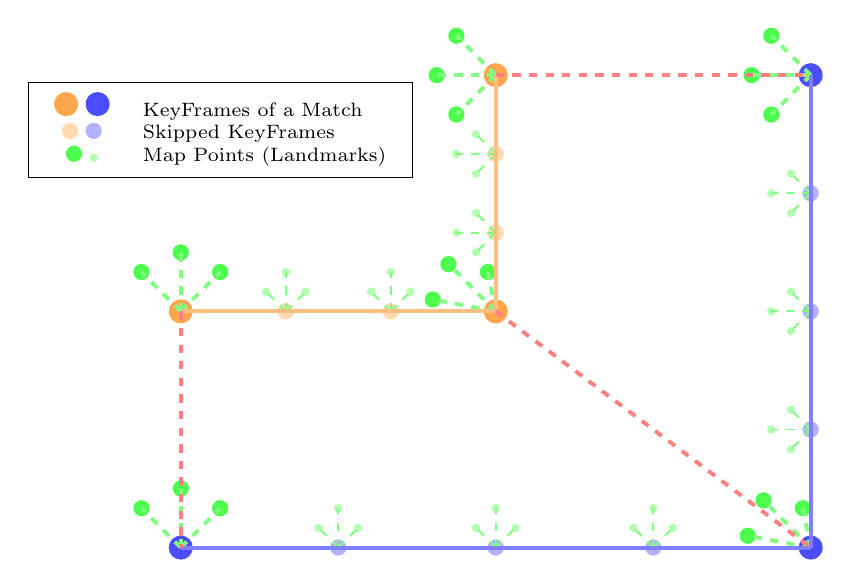
\begin{tikzpicture}
    \coordinate (A1) at (0, 3);
    \coordinate (A1MP1) at (-0.5, 3.5);
    \coordinate (A1MP2) at (0, 3.75);
    \coordinate (A1MP3) at (0.5, 3.5);

    \coordinate (AB11) at (4/3, 3);
    \coordinate (AB11MP1) at (-0.25+4/3, 3.25);
    \coordinate (AB11MP2) at (4/3, 3.5);
    \coordinate (AB11MP3) at (0.25+4/3, 3.25);

    \coordinate (AB12) at (8/3, 3);
    \coordinate (AB12MP1) at (-0.25+8/3, 3.25);
    \coordinate (AB12MP2) at (8/3, 3.5);
    \coordinate (AB12MP3) at (0.25+8/3, 3.25);

    \coordinate (B1) at (4, 3);
    \coordinate (B1MP1) at (3.2, 3.15);
    \coordinate (B1MP2) at (3.4, 3.6);
    \coordinate (B1MP3) at (3.9, 3.5);

    \coordinate (BC11) at (4, 4);
    \coordinate (BC11MP1) at (3.75, 4.25);
    \coordinate (BC11MP2) at (3.5, 4.0);
    \coordinate (BC11MP3) at (3.75, 3.75);

    \coordinate (BC12) at (4, 5);
    \coordinate (BC12MP1) at (3.75, 5.25);
    \coordinate (BC12MP2) at (3.5, 5.0);
    \coordinate (BC12MP3) at (3.75, 4.75);

    \coordinate (C1) at (4, 6);
    \coordinate (C1MP1) at (3.5, 6.5);
    \coordinate (C1MP2) at (3.25, 6.0);
    \coordinate (C1MP3) at (3.5, 5.5);

    \coordinate (A2) at (0, 0);
    \coordinate (A2MP1) at (-0.5, 0.5);
    \coordinate (A2MP2) at (0, 0.75);
    \coordinate (A2MP3) at (0.5, 0.5);

    \coordinate (AB21) at (2, 0);
    \coordinate (AB21MP1) at (1.75, 0.25);
    \coordinate (AB21MP2) at (2, 0.5);
    \coordinate (AB21MP3) at (2.25, 0.25);

    \coordinate (AB22) at (4, 0);
    \coordinate (AB22MP1) at (3.75, 0.25);
    \coordinate (AB22MP2) at (4, 0.5);
    \coordinate (AB22MP3) at (4.25, 0.25);

    \coordinate (AB23) at (6, 0);
    \coordinate (AB23MP1) at (5.75, 0.25);
    \coordinate (AB23MP2) at (6, 0.5);
    \coordinate (AB23MP3) at (6.25, 0.25);

    \coordinate (B2) at (8, 0);
    \coordinate (B2MP1) at (7.2, 0.15);
    \coordinate (B2MP2) at (7.4, 0.6);
    \coordinate (B2MP3) at (7.9, 0.5);

    \coordinate (BC21) at (8, 1.5);
    \coordinate (BC21MP1) at (7.75, 1.75);
    \coordinate (BC21MP2) at (7.5, 1.5);
    \coordinate (BC21MP3) at (7.75, 1.25);

    \coordinate (BC22) at (8, 3);
    \coordinate (BC22MP1) at (7.75, 3.25);
    \coordinate (BC22MP2) at (7.5, 3.0);
    \coordinate (BC22MP3) at (7.75, 2.75);

    \coordinate (BC23) at (8, 4.5);
    \coordinate (BC23MP1) at (7.75, 4.75);
    \coordinate (BC23MP2) at (7.5, 4.5);
    \coordinate (BC23MP3) at (7.75, 4.25);

    \coordinate (C2) at (8, 6);
    \coordinate (C2MP1) at (7.5, 6.5);
    \coordinate (C2MP2) at (7.25, 6.0);
    \coordinate (C2MP3) at (7.5, 5.5);

    \node [fill=orange!70, circle,inner sep=3pt, text width=0.1mm] at (A1) {};
    \node [fill=green!70, circle,inner sep=2pt, text width=0.1mm] at (A1MP1) {};
    \node [fill=green!70, circle,inner sep=2pt, text width=0.1mm] at (A1MP2) {};
    \node [fill=green!70, circle,inner sep=2pt, text width=0.1mm] at (A1MP3) {};
    \draw [green!50, dashed, line width=0.05cm] (A1) to (A1MP1);
    \draw [green!50, dashed, line width=0.05cm] (A1) to (A1MP2);
    \draw [green!50, dashed, line width=0.05cm] (A1) to (A1MP3);

    \node [fill=orange!30, circle,inner sep=2pt, text width=0.1mm] at (AB11) {};
    \node [fill=green!30, circle,inner sep=1pt, text width=0.1mm] at (AB11MP1) {};
    \node [fill=green!30, circle,inner sep=1pt, text width=0.1mm] at (AB11MP2) {};
    \node [fill=green!30, circle,inner sep=1pt, text width=0.1mm] at (AB11MP3) {};
    \draw [green!50, dashed, line width=0.025cm] (AB11) to (AB11MP1);
    \draw [green!50, dashed, line width=0.025cm] (AB11) to (AB11MP2);
    \draw [green!50, dashed, line width=0.025cm] (AB11) to (AB11MP3);

    \node [fill=orange!30, circle,inner sep=2pt, text width=0.1mm] at (AB12) {};
    \node [fill=green!30, circle,inner sep=1pt, text width=0.1mm] at (AB12MP1) {};
    \node [fill=green!30, circle,inner sep=1pt, text width=0.1mm] at (AB12MP2) {};
    \node [fill=green!30, circle,inner sep=1pt, text width=0.1mm] at (AB12MP3) {};
    \draw [green!50, dashed, line width=0.025cm] (AB12) to (AB12MP1);
    \draw [green!50, dashed, line width=0.025cm] (AB12) to (AB12MP2);
    \draw [green!50, dashed, line width=0.025cm] (AB12) to (AB12MP3);

    \node [fill=orange!70, circle, inner sep=3pt, text width=0.1mm] at (B1) {};
    \node [fill=green!70, circle, inner sep=2pt, text width=0.1mm] at (B1MP1) {};
    \node [fill=green!70, circle, inner sep=2pt, text width=0.1mm] at (B1MP2) {};
    \node [fill=green!70, circle, inner sep=2pt, text width=0.1mm] at (B1MP3) {};
    \draw [green!50, dashed, line width=0.05cm] (B1) to (B1MP1);
    \draw [green!50, dashed, line width=0.05cm] (B1) to (B1MP2);
    \draw [green!50, dashed, line width=0.05cm] (B1) to (B1MP3);

    \node [fill=orange!30, circle, inner sep=2pt, text width=0.1mm] at (BC11) {};
    \node [fill=green!30, circle,inner sep=1pt, text width=0.1mm] at (BC11MP1) {};
    \node [fill=green!30, circle,inner sep=1pt, text width=0.1mm] at (BC11MP2) {};
    \node [fill=green!30, circle,inner sep=1pt, text width=0.1mm] at (BC11MP3) {};
    \draw [green!50, dashed, line width=0.025cm] (BC11) to (BC11MP1);
    \draw [green!50, dashed, line width=0.025cm] (BC11) to (BC11MP2);
    \draw [green!50, dashed, line width=0.025cm] (BC11) to (BC11MP3);

    \node [fill=orange!30, circle, inner sep=2pt, text width=0.1mm] at (BC12) {};
    \node [fill=green!30, circle,inner sep=1pt, text width=0.1mm] at (BC12MP1) {};
    \node [fill=green!30, circle,inner sep=1pt, text width=0.1mm] at (BC12MP2) {};
    \node [fill=green!30, circle,inner sep=1pt, text width=0.1mm] at (BC12MP3) {};
    \draw [green!50, dashed, line width=0.025cm] (BC12) to (BC12MP1);
    \draw [green!50, dashed, line width=0.025cm] (BC12) to (BC12MP2);
    \draw [green!50, dashed, line width=0.025cm] (BC12) to (BC12MP3);

    \node [fill=orange!70, circle,inner sep=3pt, text width=0.1mm] at (C1) {};
    \node [fill=green!70, circle, inner sep=2pt, text width=0.1mm] at (C1MP1) {};
    \node [fill=green!70, circle, inner sep=2pt, text width=0.1mm] at (C1MP2) {};
    \node [fill=green!70, circle, inner sep=2pt, text width=0.1mm] at (C1MP3) {};
    \draw [green!50, dashed, line width=0.05cm] (C1) to (C1MP1);
    \draw [green!50, dashed, line width=0.05cm] (C1) to (C1MP2);
    \draw [green!50, dashed, line width=0.05cm] (C1) to (C1MP3);

    \node [fill=blue!70, circle,inner sep=3pt, text width=0.1mm] at (A2) {};
    \node [fill=green!70, circle,inner sep=2pt, text width=0.1mm] at (A2MP1) {};
    \node [fill=green!70, circle,inner sep=2pt, text width=0.1mm] at (A2MP2) {};
    \node [fill=green!70, circle,inner sep=2pt, text width=0.1mm] at (A2MP3) {};
    \draw [green!50, dashed, line width=0.05cm] (A2) to (A2MP1);
    \draw [green!50, dashed, line width=0.05cm] (A2) to (A2MP2);
    \draw [green!50, dashed, line width=0.05cm] (A2) to (A2MP3);

    \node [fill=blue!30, circle,inner sep=2pt, text width=0.1mm] at (AB21) {};
    \node [fill=green!30, circle,inner sep=1pt, text width=0.1mm] at (AB21MP1) {};
    \node [fill=green!30, circle,inner sep=1pt, text width=0.1mm] at (AB21MP2) {};
    \node [fill=green!30, circle,inner sep=1pt, text width=0.1mm] at (AB21MP3) {};
    \draw [green!50, dashed, line width=0.025cm] (AB21) to (AB21MP1);
    \draw [green!50, dashed, line width=0.025cm] (AB21) to (AB21MP2);
    \draw [green!50, dashed, line width=0.025cm] (AB21) to (AB21MP3);

    \node [fill=blue!30, circle,inner sep=2pt, text width=0.1mm] at (AB22) {};
    \node [fill=green!30, circle,inner sep=1pt, text width=0.1mm] at (AB22MP1) {};
    \node [fill=green!30, circle,inner sep=1pt, text width=0.1mm] at (AB22MP2) {};
    \node [fill=green!30, circle,inner sep=1pt, text width=0.1mm] at (AB22MP3) {};
    \draw [green!50, dashed, line width=0.025cm] (AB22) to (AB22MP1);
    \draw [green!50, dashed, line width=0.025cm] (AB22) to (AB22MP2);
    \draw [green!50, dashed, line width=0.025cm] (AB22) to (AB22MP3);

    \node [fill=blue!30, circle,inner sep=2pt, text width=0.1mm] at (AB23) {};
    \node [fill=green!30, circle,inner sep=1pt, text width=0.1mm] at (AB23MP1) {};
    \node [fill=green!30, circle,inner sep=1pt, text width=0.1mm] at (AB23MP2) {};
    \node [fill=green!30, circle,inner sep=1pt, text width=0.1mm] at (AB23MP3) {};
    \draw [green!50, dashed, line width=0.025cm] (AB23) to (AB23MP1);
    \draw [green!50, dashed, line width=0.025cm] (AB23) to (AB23MP2);
    \draw [green!50, dashed, line width=0.025cm] (AB23) to (AB23MP3);

    \node [fill=blue!70, circle,inner sep=3pt, text width=0.1mm] at (B2) {};
    \node [fill=green!70, circle,inner sep=2pt, text width=0.1mm] at (B2MP1) {};
    \node [fill=green!70, circle,inner sep=2pt, text width=0.1mm] at (B2MP2) {};
    \node [fill=green!70, circle,inner sep=2pt, text width=0.1mm] at (B2MP3) {};
    \draw [green!50, dashed, line width=0.05cm] (B2) to (B2MP1);
    \draw [green!50, dashed, line width=0.05cm] (B2) to (B2MP2);
    \draw [green!50, dashed, line width=0.05cm] (B2) to (B2MP3);

    \node [fill=blue!30, circle,inner sep=2pt, text width=0.1mm] at (BC21) {};
    \node [fill=green!30, circle,inner sep=1pt, text width=0.1mm] at (BC21MP1) {};
    \node [fill=green!30, circle,inner sep=1pt, text width=0.1mm] at (BC21MP2) {};
    \node [fill=green!30, circle,inner sep=1pt, text width=0.1mm] at (BC21MP3) {};
    \draw [green!50, dashed, line width=0.025cm] (BC21) to (BC21MP1);
    \draw [green!50, dashed, line width=0.025cm] (BC21) to (BC21MP2);
    \draw [green!50, dashed, line width=0.025cm] (BC21) to (BC21MP3);

    \node [fill=blue!30, circle,inner sep=2pt, text width=0.1mm] at (BC22) {};
    \node [fill=green!30, circle,inner sep=1pt, text width=0.1mm] at (BC22MP1) {};
    \node [fill=green!30, circle,inner sep=1pt, text width=0.1mm] at (BC22MP2) {};
    \node [fill=green!30, circle,inner sep=1pt, text width=0.1mm] at (BC22MP3) {};
    \draw [green!50, dashed, line width=0.025cm] (BC22) to (BC22MP1);
    \draw [green!50, dashed, line width=0.025cm] (BC22) to (BC22MP2);
    \draw [green!50, dashed, line width=0.025cm] (BC22) to (BC22MP3);
    
    \node [fill=blue!30, circle,inner sep=2pt, text width=0.1mm] at (BC23) {};
    \node [fill=green!30, circle,inner sep=1pt, text width=0.1mm] at (BC23MP1) {};
    \node [fill=green!30, circle,inner sep=1pt, text width=0.1mm] at (BC23MP2) {};
    \node [fill=green!30, circle,inner sep=1pt, text width=0.1mm] at (BC23MP3) {};
    \draw [green!50, dashed, line width=0.025cm] (BC23) to (BC23MP1);
    \draw [green!50, dashed, line width=0.025cm] (BC23) to (BC23MP2);
    \draw [green!50, dashed, line width=0.025cm] (BC23) to (BC23MP3);

    \node [fill=blue!70, circle,inner sep=3pt, text width=0.1mm] at (C2) {};
    \node [fill=green!70, circle, inner sep=2pt, text width=0.1mm] at (C2MP1) {};
    \node [fill=green!70, circle, inner sep=2pt, text width=0.1mm] at (C2MP2) {};
    \node [fill=green!70, circle, inner sep=2pt, text width=0.1mm] at (C2MP3) {};
    \draw [green!50, dashed, line width=0.05cm] (C2) to (C2MP1);
    \draw [green!50, dashed, line width=0.05cm] (C2) to (C2MP2);
    \draw [green!50, dashed, line width=0.05cm] (C2) to (C2MP3);

    \draw [orange!50, line width=0.05cm] (A1) to (B1);
    \draw [orange!50, line width=0.05cm] (B1) to (C1);
    \draw [blue!50, line width=0.05cm] (A2) to (B2);
    \draw [blue!50, line width=0.05cm] (B2) to (C2);

    \draw [red!50, line width=0.05cm, dashed] (A1) to (A2);
    \draw [red!50, line width=0.05cm, dashed] (B1) to (B2);
    \draw [red!50, line width=0.05cm, dashed] (C1) to (C2);

    \node[draw] at (0.5, 5.3)
    {
    \scriptsize
    \begin{tabular}{cl}
      \tikz\node[fill=orange!70, circle,inner sep=3pt, text width=0.1mm] {}; \tikz\node[fill=blue!70, circle,inner sep=3pt, text width=0.1mm] {}; & KeyFrames of a Match \\
      \tikz\node[fill=orange!30, circle,inner sep=2pt, text width=0.1mm] {}; \tikz\node[fill=blue!30, circle,inner sep=2pt, text width=0.1mm] {}; & Skipped KeyFrames \\
      \tikz\node [fill=green!70, circle, inner sep=2pt, text width=0.1mm] {}; \tikz\node[fill=green!30, circle,inner sep=1pt, text width=0.1mm] {}; & Map Points (Landmarks)
    \end{tabular}
    };
  \end{tikzpicture}
  \caption{Last \ac{KFM}}
  \label{fig:newapproach6}
\end{figure}

After the last \ac{KFM} was detected, the maps will be aligned with the transformation $T$ from the first \ac{KFM} and the \acp{MP} of the \acp{KF} belonging to a \ac{KFM} are fused, as shown in \autoref{fig:newapproach7}.

\begin{figure}[H]
  \centering
  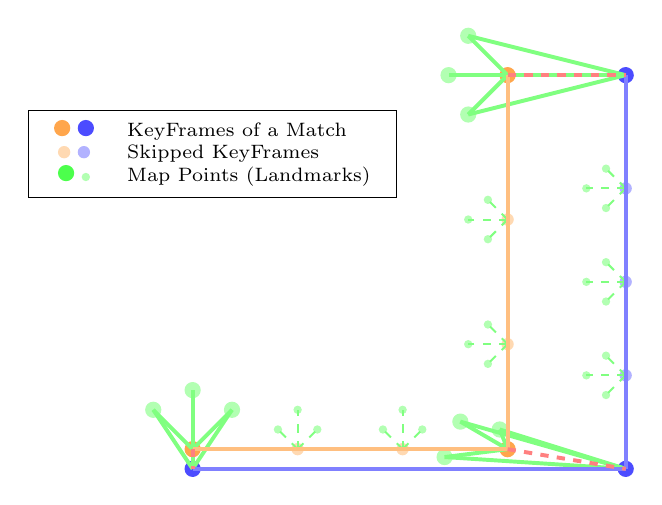
\begin{tikzpicture}
    \coordinate (A1) at (0, 0.25);
    \coordinate (A1MP1) at (-0.5, 0.75);
    \coordinate (A1MP2) at (0, 1.0);
    \coordinate (A1MP3) at (0.5, 0.75);

    \coordinate (AB11) at (4/3, 0.25);
    \coordinate (AB11MP1) at (-0.25+4/3, 0.5);
    \coordinate (AB11MP2) at (4/3, 0.75);
    \coordinate (AB11MP3) at (0.25+4/3, 0.5);

    \coordinate (AB12) at (8/3, 0.25);
    \coordinate (AB12MP1) at (-0.25+8/3, 0.5);
    \coordinate (AB12MP2) at (8/3, 0.75);
    \coordinate (AB12MP3) at (0.25+8/3, 0.5);

    \coordinate (B1) at (4, 0.25);
    \coordinate (B1MP1) at (3.2, 0.15);
    \coordinate (B1MP2) at (3.4, 0.6);
    \coordinate (B1MP3) at (3.9, 0.5);

    \coordinate (BC11) at (4, 4.75/3);
    \coordinate (BC11MP1) at (3.75, 4.75/3 + 0.25);
    \coordinate (BC11MP2) at (3.5, 4.75/3);
    \coordinate (BC11MP3) at (3.75, 4.75/3 - 0.25);

    \coordinate (BC12) at (4, 4.75/1.5);
    \coordinate (BC12MP1) at (3.75, 4.75/1.5 + 0.25);
    \coordinate (BC12MP2) at (3.5, 4.75/1.5);
    \coordinate (BC12MP3) at (3.75, 4.75/1.5 - 0.25);

    \coordinate (C1) at (4, 5);
    \coordinate (C1MP1) at (3.5, 5.5);
    \coordinate (C1MP2) at (3.25, 5.0);
    \coordinate (C1MP3) at (3.5, 4.5);

    \coordinate (A2) at (0, 0);

    \coordinate (B2) at (5.5, 0);

    \coordinate (BC21) at (5.5, 4.75/4);
    \coordinate (BC21MP1) at (5.25, 4.75/4 + 0.25);
    \coordinate (BC21MP2) at (5.0, 4.75/4);
    \coordinate (BC21MP3) at (5.25, 4.75/4 - 0.25);

    \coordinate (BC22) at (5.5, 4.75/2);
    \coordinate (BC22MP1) at (5.25, 4.75/2 + 0.25);
    \coordinate (BC22MP2) at (5.0, 4.75/2);
    \coordinate (BC22MP3) at (5.25, 4.75/2 - 0.25);

    \coordinate (BC23) at (5.5, 3*4.75/4);
    \coordinate (BC23MP1) at (5.25, 3*4.75/4 + 0.25);
    \coordinate (BC23MP2) at (5.0, 3*4.75/4);
    \coordinate (BC23MP3) at (5.25, 3*4.75/4 - 0.25);

    \coordinate (C12) at (4.5, 5.0);
    \coordinate (C2) at (5.5, 5);

    \node [fill=orange!70, circle,inner sep=2pt, text width=0.1mm] at (A1) {};
    \node [fill=green!30, circle,inner sep=2pt, text width=0.1mm] at (A1MP1) {};
    \node [fill=green!30, circle,inner sep=2pt, text width=0.1mm] at (A1MP2) {};
    \node [fill=green!30, circle,inner sep=2pt, text width=0.1mm] at (A1MP3) {};
    \draw [green!50, line width=0.05cm] (A1) to (A1MP1);
    \draw [green!50, line width=0.05cm] (A1) to (A1MP2);
    \draw [green!50, line width=0.05cm] (A1) to (A1MP3);

    \node [fill=orange!30, circle,inner sep=1.5pt, text width=0.1mm] at (AB11) {};
    \node [fill=green!30, circle,inner sep=1pt, text width=0.1mm] at (AB11MP1) {};
    \node [fill=green!30, circle,inner sep=1pt, text width=0.1mm] at (AB11MP2) {};
    \node [fill=green!30, circle,inner sep=1pt, text width=0.1mm] at (AB11MP3) {};
    \draw [green!50, dashed, line width=0.025cm] (AB11) to (AB11MP1);
    \draw [green!50, dashed, line width=0.025cm] (AB11) to (AB11MP2);
    \draw [green!50, dashed, line width=0.025cm] (AB11) to (AB11MP3);

    \node [fill=orange!30, circle,inner sep=1.5pt, text width=0.1mm] at (AB12) {};
    \node [fill=green!30, circle,inner sep=1pt, text width=0.1mm] at (AB12MP1) {};
    \node [fill=green!30, circle,inner sep=1pt, text width=0.1mm] at (AB12MP2) {};
    \node [fill=green!30, circle,inner sep=1pt, text width=0.1mm] at (AB12MP3) {};
    \draw [green!50, dashed, line width=0.025cm] (AB12) to (AB12MP1);
    \draw [green!50, dashed, line width=0.025cm] (AB12) to (AB12MP2);
    \draw [green!50, dashed, line width=0.025cm] (AB12) to (AB12MP3);

    \node [fill=orange!70, circle,inner sep=2pt, text width=0.1mm] at (B1) {};
    \node [fill=green!30, circle, inner sep=2pt, text width=0.1mm] at (B1MP1) {};
    \node [fill=green!30, circle, inner sep=2pt, text width=0.1mm] at (B1MP2) {};
    \node [fill=green!30, circle, inner sep=2pt, text width=0.1mm] at (B1MP3) {};
    \draw [green!50, line width=0.05cm] (B1) to (B1MP1);
    \draw [green!50, line width=0.05cm] (B1) to (B1MP2);
    \draw [green!50, line width=0.05cm] (B1) to (B1MP3);

    \node [fill=orange!30, circle, inner sep=1.5pt, text width=0.1mm] at (BC11) {};
    \node [fill=green!30, circle,inner sep=1pt, text width=0.1mm] at (BC11MP1) {};
    \node [fill=green!30, circle,inner sep=1pt, text width=0.1mm] at (BC11MP2) {};
    \node [fill=green!30, circle,inner sep=1pt, text width=0.1mm] at (BC11MP3) {};
    \draw [green!50, dashed, line width=0.025cm] (BC11) to (BC11MP1);
    \draw [green!50, dashed, line width=0.025cm] (BC11) to (BC11MP2);
    \draw [green!50, dashed, line width=0.025cm] (BC11) to (BC11MP3);

    \node [fill=orange!30, circle, inner sep=1.5pt, text width=0.1mm] at (BC12) {};
    \node [fill=green!30, circle,inner sep=1pt, text width=0.1mm] at (BC12MP1) {};
    \node [fill=green!30, circle,inner sep=1pt, text width=0.1mm] at (BC12MP2) {};
    \node [fill=green!30, circle,inner sep=1pt, text width=0.1mm] at (BC12MP3) {};
    \draw [green!50, dashed, line width=0.025cm] (BC12) to (BC12MP1);
    \draw [green!50, dashed, line width=0.025cm] (BC12) to (BC12MP2);
    \draw [green!50, dashed, line width=0.025cm] (BC12) to (BC12MP3);

    \node [fill=orange!70, circle,inner sep=2pt, text width=0.1mm] at (C1) {};
    \node [fill=green!30, circle, inner sep=2pt, text width=0.1mm] at (C1MP1) {};
    \node [fill=green!30, circle, inner sep=2pt, text width=0.1mm] at (C1MP2) {};
    \node [fill=green!30, circle, inner sep=2pt, text width=0.1mm] at (C1MP3) {};
    \draw [green!50, line width=0.05cm] (C1) to (C1MP1);
    \draw [green!50, line width=0.05cm] (C1) to (C1MP2);
    \draw [green!50, line width=0.05cm] (C1) to (C1MP3);

    \node [fill=blue!70, circle,inner sep=2pt, text width=0.1mm] at (A2) {};
    \draw [green!50, line width=0.05cm] (A2) to (A1MP1);
    \draw [green!50, line width=0.05cm] (A2) to (A1MP2);
    \draw [green!50, line width=0.05cm] (A2) to (A1MP3);

    \node [fill=blue!70, circle,inner sep=2pt, text width=0.1mm] at (B2) {};
    \draw [green!50, line width=0.05cm] (B2) to (B1MP1);
    \draw [green!50, line width=0.05cm] (B2) to (B1MP2);
    \draw [green!50, line width=0.05cm] (B2) to (B1MP3);

    \node [fill=blue!30, circle,inner sep=1.5pt, text width=0.1mm] at (BC21) {};
    \node [fill=green!30, circle,inner sep=1pt, text width=0.1mm] at (BC21MP1) {};
    \node [fill=green!30, circle,inner sep=1pt, text width=0.1mm] at (BC21MP2) {};
    \node [fill=green!30, circle,inner sep=1pt, text width=0.1mm] at (BC21MP3) {};
    \draw [green!50, dashed, line width=0.025cm] (BC21) to (BC21MP1);
    \draw [green!50, dashed, line width=0.025cm] (BC21) to (BC21MP2);
    \draw [green!50, dashed, line width=0.025cm] (BC21) to (BC21MP3);

    \node [fill=blue!30, circle,inner sep=1.5pt, text width=0.1mm] at (BC22) {};
    \node [fill=green!30, circle,inner sep=1pt, text width=0.1mm] at (BC22MP1) {};
    \node [fill=green!30, circle,inner sep=1pt, text width=0.1mm] at (BC22MP2) {};
    \node [fill=green!30, circle,inner sep=1pt, text width=0.1mm] at (BC22MP3) {};
    \draw [green!50, dashed, line width=0.025cm] (BC22) to (BC22MP1);
    \draw [green!50, dashed, line width=0.025cm] (BC22) to (BC22MP2);
    \draw [green!50, dashed, line width=0.025cm] (BC22) to (BC22MP3);

    \node [fill=blue!30, circle,inner sep=1.5pt, text width=0.1mm] at (BC23) {};
    \node [fill=green!30, circle,inner sep=1pt, text width=0.1mm] at (BC23MP1) {};
    \node [fill=green!30, circle,inner sep=1pt, text width=0.1mm] at (BC23MP2) {};
    \node [fill=green!30, circle,inner sep=1pt, text width=0.1mm] at (BC23MP3) {};
    \draw [green!50, dashed, line width=0.025cm] (BC23) to (BC23MP1);
    \draw [green!50, dashed, line width=0.025cm] (BC23) to (BC23MP2);
    \draw [green!50, dashed, line width=0.025cm] (BC23) to (BC23MP3);

    \node [fill=blue!70, circle,inner sep=2pt, text width=0.1mm] at (C2) {};
    \draw [green!50, line width=0.05cm] (C2) to (C1MP1);
    \draw [green!50, line width=0.05cm] (C2) to (C1MP2);
    \draw [green!50, line width=0.05cm] (C2) to (C1MP3);

    \draw [orange!50, line width=0.05cm] (A1) to (B1);
    \draw [orange!50, line width=0.05cm] (B1) to (C1);
    \draw [blue!50, line width=0.05cm] (A2) to (B2);
    \draw [blue!50, line width=0.05cm] (B2) to (C2);

    \draw [red!50, line width=0.05cm, dashed] (A1) to (A2);
    \draw [red!50, line width=0.05cm, dashed] (B1) to (B2);
    \draw [red!50, line width=0.05cm, dashed] (C1) to (C2);

    \node[draw] at (0.25, 4.0)
    {
      \scriptsize
      \begin{tabular}{cl}
        \tikz\node[fill=orange!70, circle,inner sep=2pt, text width=0.1mm] {}; \tikz\node[fill=blue!70, circle,inner sep=2pt, text width=0.1mm] {}; & KeyFrames of a Match \\
        \tikz\node[fill=orange!30, circle,inner sep=1.5pt, text width=0.1mm] {}; \tikz\node[fill=blue!30, circle,inner sep=1.5pt, text width=0.1mm] {}; & Skipped KeyFrames \\
        \tikz\node [fill=green!70, circle, inner sep=2pt, text width=0.1mm] {}; \tikz\node[fill=green!30, circle,inner sep=1pt, text width=0.1mm] {}; & Map Points (Landmarks)
      \end{tabular}
    };
  \end{tikzpicture}%}
  \caption{Maps aligned}
  \label{fig:newapproach7}
\end{figure}

After the two maps are aligned (possibly still with some miss alignment as in \autoref{fig:newapproach7}), the \ac{PGO} will be performed which optimizes the poses of the \acp{KF} and afterwards the \ac{BA} will be performed which optimizes the poses of both, the \acp{KF} and the \acp{MP}.\\

The idea behind the usage of multiple \acp{KFM} was already discussed in contrary to the idea of skipping \acp{KF} after a \ac{KFM} was detected. This idea will be discussed next.

If \acp{KF} are skipped after a \ac{KFM} was detected, the next \ac{KFM} will potentially have a bigger distance to the previous \ac{KFM}. This causes that the \acp{KFM} will be more apart from each other and therefor they will cover a bigger area. The \acp{KFM} from a bigger area provide the \ac{PGO} and the \ac{BA} with more information which hopefully leads to a reduction in drift and an increased accuracy.
%\textcolor{red}{\textbf{!!!Check \ac{PGO} implementation!!!}}

To visualize the influence of this idea, \autoref{fig:kfskip1} shows the co-visibility graph of an experiment where only one \ac{KF} was skipped after a \ac{KFM} was detected. \autoref{fig:kfskip2} on the other hand shows an experiment where 10 \acp{KF} were skipped after a \ac{KFM} was detected. One can easily see, that the \acp{KFM} in \autoref{fig:kfskip2} are more apart from each other and cover a bigger area compared to the \acp{KFM} in \autoref{fig:kfskip1}.

\begin{figure}[H]
   \centering
   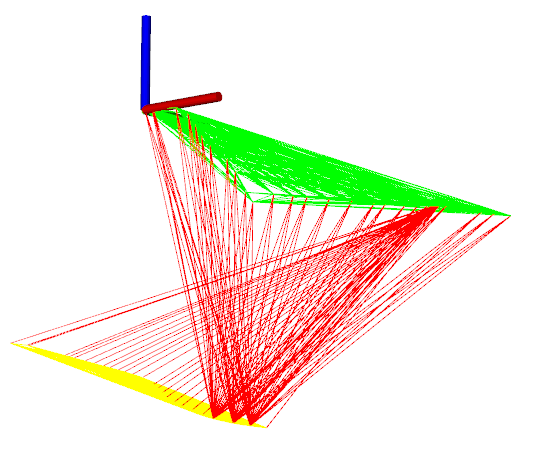
\includegraphics[width=0.75\textwidth]{images/covgraph_minHits_5_skip_1}
   \caption{One \ac{KF} skipped after a \ac{KFM} was found\\
   \textcolor{green}{green}: Co-visibility graph of first map\\ \textcolor{yellow}{yellow}: Co-visibility graph of second map\\ \textcolor{red}{red}: Co-visibility between the \acp{KFM}}
   \label{fig:kfskip1}
\end{figure}

\begin{figure}[H]
   \centering
   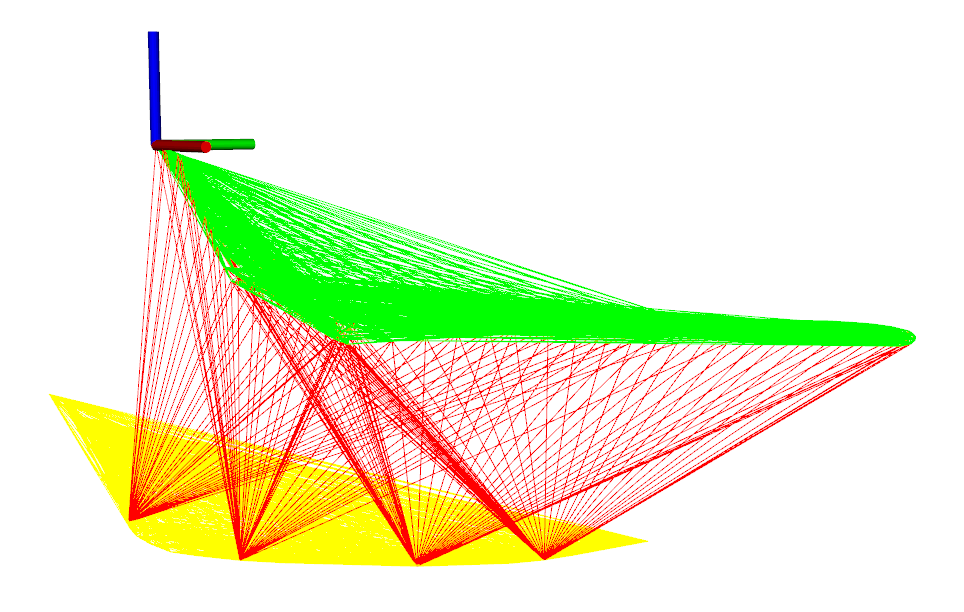
\includegraphics[width=0.75\textwidth]{images/covgraph_minHits_5_skip_10}
   \caption{10 \acp{KF} skipped after a \ac{KFM} was found\\
   \textcolor{green}{green}: Co-visibility graph of first map\\ \textcolor{yellow}{yellow}: Co-visibility graph of second map\\ \textcolor{red}{red}: Co-visibility between the \acp{KFM}}
   \label{fig:kfskip2}
\end{figure}

\section{Culling}
\label{sec:culling}

Culling is motivated by the fact, that the \ac{BA} complexity grows with the number of \acp{KF} and that it enables lifelong operation in the same environment as the number of \acp{KF} will not grow unbounded \cite{Mur-Artal2015}.

ORB-SLAM(2) \cite{Mur-Artal2015}, \cite{Mur-Artal2016} already implemented a \ac{KF} culling mechanism which works locally. As the proposed new approach uses multiple \acp{KFM} to fuse two maps, \ac{KF} culling within the fusion procedure could remove redundant \acp{KF} from a bigger area compared to the standard \ac{KF} culling approach of ORB-SLAM(2).

\subsection{Approach}

The culling of \acp{KF} is an additional step in the map fusion procedure which is executed after $n$ \acp{KFM} were found and before the maps are aligned and the \acp{MP} are fused.

The culling during the map fusion follows the same approach as the one used for the local \ac{KF} culling in ORB-SLAM(2) \cite{Mur-Artal2015}, \cite{Mur-Artal2016}: All the \acp{KF} which observe a certain percentage of \acp{MP}, the redundancy threshold, which have also been seen in at least three other \acp{KF} in the same or finer scale, are discarded.

Culling of \acp{KF} is performed for every \ac{KFM} separately. Therefore the \acp{KF} which are considered for culling per \ac{KFM} are the two \acp{KF} of the \ac{KFM} and their direct neighbors in the co-visibility graph. \autoref{fig:culling0} visualizes this, where the \textcolor{blue}{blue ellipses} indicate the direct neighbors in the co-visibility graph and the \textcolor{red}{red ellipse} surrounds all the \acp{KF} which are considered for the culling for one \ac{KFM}.

\tikzstyle{abstract}=[rectangle, draw=black, rounded corners, fill=white!40, drop shadow,
        text centered, anchor=north, text=black, text width=3cm]
\begin{figure}[H]
  \centering
%  \begin{tikzpicture}[auto]
%    \node[entity] (key frame match) {\ac{KFM}}
%      [grow=down,sibling distance=4.5cm]
%        child {node[entity] (child 1) {\ac{KF}, map 1}
%          [grow=down,sibling distance=1.2cm]
%          child {node[entity,minimum size=1cm] {\ac{KF} 1}}
%          child {node[entity,minimum size=1cm] {\ac{KF} 2}}
%          child {node[entity,minimum size=1cm] {\ac{KF} $k$}}}
%        child {node[entity] {\ac{KF}, map 2}
%          [grow=down,sibling distance=1.2cm]
%          child {node[entity,minimum size=1cm] {\ac{KF} 1}}
%          child {node[entity,minimum size=1cm] {\ac{KF} 2}}
%          child {node[entity,minimum size=1cm] {\ac{KF} $l$}}};
%
%    \draw[blue,thick,dashed] (-2.25,-2.25) ellipse (1.5 and 0.5);
%
%    \draw[blue,thick,dashed] (2.25,-2.25) ellipse (1.5 and 0.5);
%
%    \draw[red,thick,dashed] (0,-2.25) ellipse (5 and 1.5);
%  \end{tikzpicture}

%  \begin{tikzpicture}[auto]
%  \node (KFM) [abstract, rectangle split, rectangle split parts=3]
%  {
%    \textbf{\ac{KFM}}
%    \nodepart{second}\ac{KF}, map 1
%    \nodepart{third}\ac{KF}, map 2
%  };
%  \end{tikzpicture}

  \begin{tikzpicture}
    % Box representing the KFM with two KFs
    \draw (-0.1, 1.9) -- (4.1, 1.9) -- (4.1, 4) -- (-0.1, 4) -- (-0.1, 1.9);
    \node at (2, 3.5)  {\ac{KFM}};
    \node[entity] at (1, 2.5) (kfm_kf1)  {\ac{KF}, map 1};
    \node[entity] at (3, 2.5) (kfm_kf2) {\ac{KF}, map 2};

    % Co-visibility graph kfs
    \node[entity,minimum width=1cm] at (-2.0, 0.75) (kf_1) {\ac{KF} 1};
    \node[entity,minimum width=1cm] at (-0.5, 0.75) (kf_2) {\ac{KF} 2};
    \node[entity,minimum width=1cm] at (1.0, 0.75) (kf_3) {\ac{KF} $k$};

    \node[entity,minimum width=1cm] at (6.0, 0.75) (kf_4) {\ac{KF} $l$};
    \node[entity,minimum width=1cm] at (4.5, 0.75) (kf_5) {\ac{KF} 2};
    \node[entity,minimum width=1cm] at (3.0, 0.75) (kf_6) {\ac{KF} 1};

    % Edges between kfm kfs and co-visibility graph kfs
    \draw (kfm_kf1.south) -- (kf_1.north);
    \draw (kfm_kf1.south) -- (kf_2.north);
    \draw (kfm_kf1.south) -- (kf_3.north);
    \draw (kfm_kf2.south) -- (kf_4.north);
    \draw (kfm_kf2.south) -- (kf_5.north);
    \draw (kfm_kf2.south) -- (kf_6.north);

    % Ellipses
    \draw[blue,thick,dashed] (-0.5, 1.625) ellipse (2.25 and 0.75);
    \draw[blue,thick,dashed] (4.5, 1.625) ellipse (2.25 and 0.75);
    \draw[red,thick,dashed] (2.0, 1.4) ellipse (5 and 1.75);
  \end{tikzpicture}
  \caption{\ac{KFM} with its \acp{KF} and their direct neighbors in the \textcolor{blue}{co-visibility graph}}
  \label{fig:culling0}
\end{figure}

To illustrate the culling procedure, \autoref{fig:culling1} shows the maps of two robots in a toy example.

\begin{figure}[H]
  \centering
  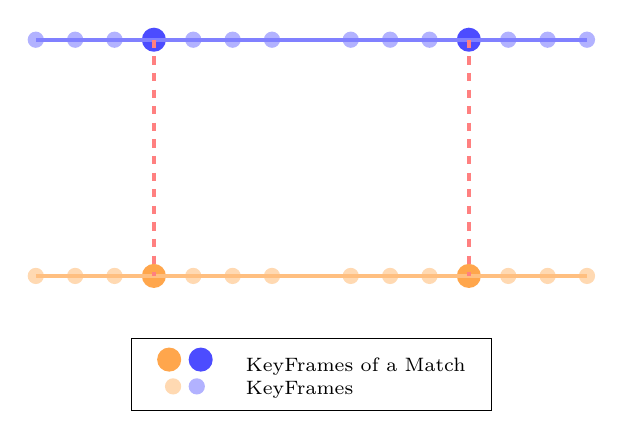
\begin{tikzpicture}[auto]
    \coordinate (A1) at (-0.5, 0);
    \coordinate (KFM11) at (1, 0);
    \coordinate (A1MP1) at (-0.5, 0);
    \coordinate (A1MP2) at (0, 0);
    \coordinate (A1MP3) at (0.5, 0);
    \coordinate (A1MP4) at (1.5, 0);
    \coordinate (A1MP5) at (2, 0);
    \coordinate (A1MP6) at (2.5, 0);

    \coordinate (B1) at (6.5, 0);
    \coordinate (KFM12) at (5, 0);
    \coordinate (B1MP1) at (5.5, 0);
    \coordinate (B1MP2) at (6.0, 0);
    \coordinate (B1MP3) at (6.5, 0);
    \coordinate (B1MP4) at (4.5, 0);
    \coordinate (B1MP5) at (4.0, 0);
    \coordinate (B1MP6) at (3.5, 0);

    \coordinate (A2) at (-0.5, -3);
    \coordinate (KFM21) at (1, -3);
    \coordinate (A2MP1) at (-0.5, -3);
    \coordinate (A2MP2) at (0, -3);
    \coordinate (A2MP3) at (0.5, -3);
    \coordinate (A2MP4) at (1.5, -3);
    \coordinate (A2MP5) at (2, -3);
    \coordinate (A2MP6) at (2.5, -3);

    \coordinate (B2) at (6.5, -3);
    \coordinate (KFM22) at (5, -3);
    \coordinate (B2MP1) at (5.5, -3);
    \coordinate (B2MP2) at (6.0, -3);
    \coordinate (B2MP3) at (6.5, -3);
    \coordinate (B2MP4) at (4.5, -3);
    \coordinate (B2MP5) at (4.0, -3);
    \coordinate (B2MP6) at (3.5, -3);

    \node [fill=blue!30, circle,inner sep=2pt, text width=0.1mm] at (A1MP1) {};
    \node [fill=blue!30, circle,inner sep=2pt, text width=0.1mm] at (A1MP2) {};
    \node [fill=blue!30, circle,inner sep=2pt, text width=0.1mm] at (A1MP3) {};
    \node [fill=blue!70, circle,inner sep=3pt, text width=0.1mm] at (KFM11) {};
    \node [fill=blue!30, circle,inner sep=2pt, text width=0.1mm] at (A1MP4) {};
    \node [fill=blue!30, circle,inner sep=2pt, text width=0.1mm] at (A1MP5) {};
    \node [fill=blue!30, circle,inner sep=2pt, text width=0.1mm] at (A1MP6) {};

    \node [fill=blue!30, circle,inner sep=2pt, text width=0.1mm] at (B1MP1) {};
    \node [fill=blue!30, circle,inner sep=2pt, text width=0.1mm] at (B1MP2) {};
    \node [fill=blue!30, circle,inner sep=2pt, text width=0.1mm] at (B1MP3) {};
    \node [fill=blue!70, circle,inner sep=3pt, text width=0.1mm] at (KFM12) {};
    \node [fill=blue!30, circle,inner sep=2pt, text width=0.1mm] at (B1MP4) {};
    \node [fill=blue!30, circle,inner sep=2pt, text width=0.1mm] at (B1MP5) {};
    \node [fill=blue!30, circle,inner sep=2pt, text width=0.1mm] at (B1MP6) {};

    \node [fill=orange!30, circle,inner sep=2pt, text width=0.1mm] at (A2MP1) {};
    \node [fill=orange!30, circle,inner sep=2pt, text width=0.1mm] at (A2MP2) {};
    \node [fill=orange!30, circle,inner sep=2pt, text width=0.1mm] at (A2MP3) {};
    \node [fill=orange!70, circle,inner sep=3pt, text width=0.1mm] at (KFM21) {};
    \node [fill=orange!30, circle,inner sep=2pt, text width=0.1mm] at (A2MP4) {};
    \node [fill=orange!30, circle,inner sep=2pt, text width=0.1mm] at (A2MP5) {};
    \node [fill=orange!30, circle,inner sep=2pt, text width=0.1mm] at (A2MP6) {};

    \node [fill=orange!30, circle,inner sep=2pt, text width=0.1mm] at (B2MP1) {};
    \node [fill=orange!30, circle,inner sep=2pt, text width=0.1mm] at (B2MP2) {};
    \node [fill=orange!30, circle,inner sep=2pt, text width=0.1mm] at (B2MP3) {};
    \node [fill=orange!70, circle,inner sep=3pt, text width=0.1mm] at (KFM22) {};
    \node [fill=orange!30, circle,inner sep=2pt, text width=0.1mm] at (B2MP4) {};
    \node [fill=orange!30, circle,inner sep=2pt, text width=0.1mm] at (B2MP5) {};
    \node [fill=orange!30, circle,inner sep=2pt, text width=0.1mm] at (B2MP6) {};

    \draw [blue!50, line width=0.05cm] (A1) to (B1);
    \draw [orange!50, line width=0.05cm] (A2) to (B2);

    \draw [red!50, line width=0.05cm, dashed] (KFM11) to (KFM21);
    \draw [red!50, line width=0.05cm, dashed] (KFM12) to (KFM22);

    \node[draw] at (3.0, -4.25)
    {
    \scriptsize
    \begin{tabular}{cl}
      \tikz\node[fill=orange!70, circle,inner sep=3pt, text width=0.1mm] {}; \tikz\node[fill=blue!70, circle,inner sep=3pt, text width=0.1mm] {}; & KeyFrames of a Match \\
      \tikz\node[fill=orange!30, circle,inner sep=2.0pt, text width=0.1mm] {}; \tikz\node[fill=blue!30, circle,inner sep=2.0pt, text width=0.1mm] {}; & KeyFrames \\
    \end{tabular}
    };
    \end{tikzpicture}
  \caption{Toy example of the maps of two clients}
  \label{fig:culling1}
\end{figure}

\autoref{fig:culling2} then shows the \acp{KF} which are directly connected to the \acp{KF} of a \ac{KFM} indicated by dashed rectangles.

\begin{figure}[H]
  \centering
  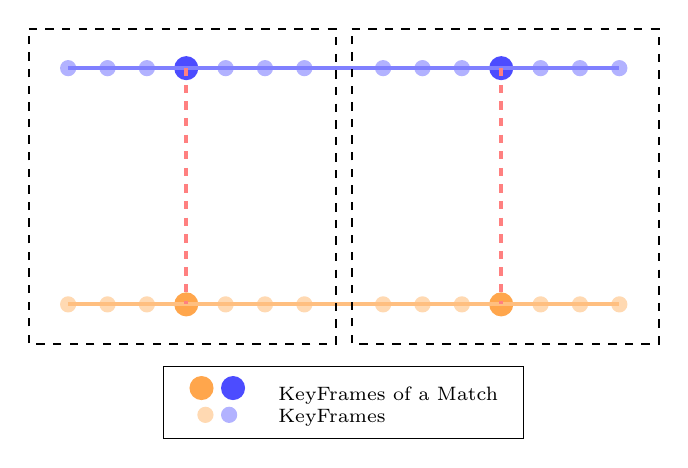
\begin{tikzpicture}[auto]
    \coordinate (A1) at (-0.5, 0);
    \coordinate (KFM11) at (1, 0);
    \coordinate (A1MP1) at (-0.5, 0);
    \coordinate (A1MP2) at (0, 0);
    \coordinate (A1MP3) at (0.5, 0);
    \coordinate (A1MP4) at (1.5, 0);
    \coordinate (A1MP5) at (2, 0);
    \coordinate (A1MP6) at (2.5, 0);

    \coordinate (B1) at (6.5, 0);
    \coordinate (KFM12) at (5, 0);
    \coordinate (B1MP1) at (5.5, 0);
    \coordinate (B1MP2) at (6.0, 0);
    \coordinate (B1MP3) at (6.5, 0);
    \coordinate (B1MP4) at (4.5, 0);
    \coordinate (B1MP5) at (4.0, 0);
    \coordinate (B1MP6) at (3.5, 0);

    \coordinate (A2) at (-0.5, -3);
    \coordinate (KFM21) at (1, -3);
    \coordinate (A2MP1) at (-0.5, -3);
    \coordinate (A2MP2) at (0, -3);
    \coordinate (A2MP3) at (0.5, -3);
    \coordinate (A2MP4) at (1.5, -3);
    \coordinate (A2MP5) at (2, -3);
    \coordinate (A2MP6) at (2.5, -3);

    \coordinate (B2) at (6.5, -3);
    \coordinate (KFM22) at (5, -3);
    \coordinate (B2MP1) at (5.5, -3);
    \coordinate (B2MP2) at (6.0, -3);
    \coordinate (B2MP3) at (6.5, -3);
    \coordinate (B2MP4) at (4.5, -3);
    \coordinate (B2MP5) at (4.0, -3);
    \coordinate (B2MP6) at (3.5, -3);

    \node [fill=blue!30, circle,inner sep=2pt, text width=0.1mm] at (A1MP1) {};
    \node [fill=blue!30, circle,inner sep=2pt, text width=0.1mm] at (A1MP2) {};
    \node [fill=blue!30, circle,inner sep=2pt, text width=0.1mm] at (A1MP3) {};
    \node [fill=blue!70, circle,inner sep=3pt, text width=0.1mm] at (KFM11) {};
    \node [fill=blue!30, circle,inner sep=2pt, text width=0.1mm] at (A1MP4) {};
    \node [fill=blue!30, circle,inner sep=2pt, text width=0.1mm] at (A1MP5) {};
    \node [fill=blue!30, circle,inner sep=2pt, text width=0.1mm] at (A1MP6) {};

    \node [fill=blue!30, circle,inner sep=2pt, text width=0.1mm] at (B1MP1) {};
    \node [fill=blue!30, circle,inner sep=2pt, text width=0.1mm] at (B1MP2) {};
    \node [fill=blue!30, circle,inner sep=2pt, text width=0.1mm] at (B1MP3) {};
    \node [fill=blue!70, circle,inner sep=3pt, text width=0.1mm] at (KFM12) {};
    \node [fill=blue!30, circle,inner sep=2pt, text width=0.1mm] at (B1MP4) {};
    \node [fill=blue!30, circle,inner sep=2pt, text width=0.1mm] at (B1MP5) {};
    \node [fill=blue!30, circle,inner sep=2pt, text width=0.1mm] at (B1MP6) {};

    \node [fill=orange!30, circle,inner sep=2pt, text width=0.1mm] at (A2MP1) {};
    \node [fill=orange!30, circle,inner sep=2pt, text width=0.1mm] at (A2MP2) {};
    \node [fill=orange!30, circle,inner sep=2pt, text width=0.1mm] at (A2MP3) {};
    \node [fill=orange!70, circle,inner sep=3pt, text width=0.1mm] at (KFM21) {};
    \node [fill=orange!30, circle,inner sep=2pt, text width=0.1mm] at (A2MP4) {};
    \node [fill=orange!30, circle,inner sep=2pt, text width=0.1mm] at (A2MP5) {};
    \node [fill=orange!30, circle,inner sep=2pt, text width=0.1mm] at (A2MP6) {};

    \node [fill=orange!30, circle,inner sep=2pt, text width=0.1mm] at (B2MP1) {};
    \node [fill=orange!30, circle,inner sep=2pt, text width=0.1mm] at (B2MP2) {};
    \node [fill=orange!30, circle,inner sep=2pt, text width=0.1mm] at (B2MP3) {};
    \node [fill=orange!70, circle,inner sep=3pt, text width=0.1mm] at (KFM22) {};
    \node [fill=orange!30, circle,inner sep=2pt, text width=0.1mm] at (B2MP4) {};
    \node [fill=orange!30, circle,inner sep=2pt, text width=0.1mm] at (B2MP5) {};
    \node [fill=orange!30, circle,inner sep=2pt, text width=0.1mm] at (B2MP6) {};

    \draw [blue!50, line width=0.05cm] (A1) to (B1);
    \draw [orange!50, line width=0.05cm] (A2) to (B2);

    \draw [red!50, line width=0.05cm, dashed] (KFM11) to (KFM21);
    \draw [red!50, line width=0.05cm, dashed] (KFM12) to (KFM22);

    \draw[black,thick,dashed] (-1, 0.5) -- (2.9, 0.5) -- (2.9, -3.5) -- (-1, -3.5) -- (-1, 0.5);
    \draw[black,thick,dashed] (3.1, 0.5) -- (7.0, 0.5) -- (7.0, -3.5) -- (3.1, -3.5) -- (3.1, 0.5);

    \node[draw] at (3.0, -4.25)
    {
    \scriptsize
    \begin{tabular}{cl}
      \tikz\node[fill=orange!70, circle,inner sep=3pt, text width=0.1mm] {}; \tikz\node[fill=blue!70, circle,inner sep=3pt, text width=0.1mm] {}; & KeyFrames of a Match \\
      \tikz\node[fill=orange!30, circle,inner sep=2.0pt, text width=0.1mm] {}; \tikz\node[fill=blue!30, circle,inner sep=2.0pt, text width=0.1mm] {}; & KeyFrames \\
    \end{tabular}
    };
    \end{tikzpicture}
  \caption{Two \acp{KFM} with their neighborhood}
  \label{fig:culling2}
\end{figure}

The toy example with culled \acp{KF} is shown in \autoref{fig:culling3}, where the \textcolor{red}{x} represent culled \acp{KF}.

\begin{figure}[H]
  \centering
  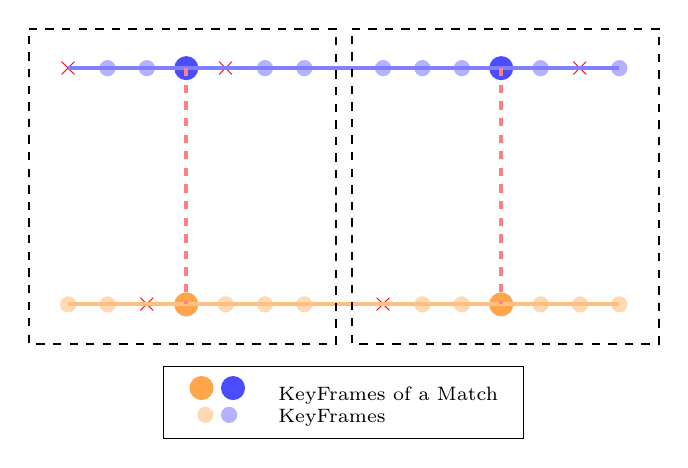
\begin{tikzpicture}[auto]
    \coordinate (A1) at (-0.5, 0);
    \coordinate (KFM11) at (1, 0);
    \coordinate (A1MP1) at (-0.5, 0);
    \coordinate (A1MP2) at (0, 0);
    \coordinate (A1MP3) at (0.5, 0);
    \coordinate (A1MP4) at (1.5, 0);
    \coordinate (A1MP5) at (2, 0);
    \coordinate (A1MP6) at (2.5, 0);

    \coordinate (B1) at (6.5, 0);
    \coordinate (KFM12) at (5, 0);
    \coordinate (B1MP1) at (5.5, 0);
    \coordinate (B1MP2) at (6.0, 0);
    \coordinate (B1MP3) at (6.5, 0);
    \coordinate (B1MP4) at (4.5, 0);
    \coordinate (B1MP5) at (4.0, 0);
    \coordinate (B1MP6) at (3.5, 0);

    \coordinate (A2) at (-0.5, -3);
    \coordinate (KFM21) at (1, -3);
    \coordinate (A2MP1) at (-0.5, -3);
    \coordinate (A2MP2) at (0, -3);
    \coordinate (A2MP3) at (0.5, -3);
    \coordinate (A2MP4) at (1.5, -3);
    \coordinate (A2MP5) at (2, -3);
    \coordinate (A2MP6) at (2.5, -3);

    \coordinate (B2) at (6.5, -3);
    \coordinate (KFM22) at (5, -3);
    \coordinate (B2MP1) at (5.5, -3);
    \coordinate (B2MP2) at (6.0, -3);
    \coordinate (B2MP3) at (6.5, -3);
    \coordinate (B2MP4) at (4.5, -3);
    \coordinate (B2MP5) at (4.0, -3);
    \coordinate (B2MP6) at (3.5, -3);

    \node [red] at (A1MP1) {$\boldsymbol{\times}$};
    \node [fill=blue!30, circle,inner sep=2pt, text width=0.1mm] at (A1MP2) {};
    \node [fill=blue!30, circle,inner sep=2pt, text width=0.1mm] at (A1MP3) {};
    \node [fill=blue!70, circle,inner sep=3pt, text width=0.1mm] at (KFM11) {};
    \node [red] at (A1MP4) {$\boldsymbol{\times}$};
    \node [fill=blue!30, circle,inner sep=2pt, text width=0.1mm] at (A1MP5) {};
    \node [fill=blue!30, circle,inner sep=2pt, text width=0.1mm] at (A1MP6) {};

    \node [fill=blue!30, circle,inner sep=2pt, text width=0.1mm] at (B1MP1) {};
    \node [red] at (B1MP2) {$\boldsymbol{\times}$};
    \node [fill=blue!30, circle,inner sep=2pt, text width=0.1mm] at (B1MP3) {};
    \node [fill=blue!70, circle,inner sep=3pt, text width=0.1mm] at (KFM12) {};
    \node [fill=blue!30, circle,inner sep=2pt, text width=0.1mm] at (B1MP4) {};
    \node [fill=blue!30, circle,inner sep=2pt, text width=0.1mm] at (B1MP5) {};
    \node [fill=blue!30, circle,inner sep=2pt, text width=0.1mm] at (B1MP6) {};

    \node [fill=orange!30, circle,inner sep=2pt, text width=0.1mm] at (A2MP1) {};
    \node [fill=orange!30, circle,inner sep=2pt, text width=0.1mm] at (A2MP2) {};
    \node [red] at (A2MP3) {$\boldsymbol{\times}$};
    \node [fill=orange!70, circle,inner sep=3pt, text width=0.1mm] at (KFM21) {};
    \node [fill=orange!30, circle,inner sep=2pt, text width=0.1mm] at (A2MP4) {};
    \node [fill=orange!30, circle,inner sep=2pt, text width=0.1mm] at (A2MP5) {};
    \node [fill=orange!30, circle,inner sep=2pt, text width=0.1mm] at (A2MP6) {};

    \node [fill=orange!30, circle,inner sep=2pt, text width=0.1mm] at (B2MP1) {};
    \node [fill=orange!30, circle,inner sep=2pt, text width=0.1mm] at (B2MP2) {};
    \node [fill=orange!30, circle,inner sep=2pt, text width=0.1mm] at (B2MP3) {};
    \node [fill=orange!70, circle,inner sep=3pt, text width=0.1mm] at (KFM22) {};
    \node [fill=orange!30, circle,inner sep=2pt, text width=0.1mm] at (B2MP4) {};
    \node [fill=orange!30, circle,inner sep=2pt, text width=0.1mm] at (B2MP5) {};
    \node [red] at (B2MP6) {$\boldsymbol{\times}$};

    \draw [blue!50, line width=0.05cm] (A1) to (B1);
    \draw [orange!50, line width=0.05cm] (A2) to (B2);

    \draw [red!50, line width=0.05cm, dashed] (KFM11) to (KFM21);
    \draw [red!50, line width=0.05cm, dashed] (KFM12) to (KFM22);

    \draw[black,thick,dashed] (-1, 0.5) -- (2.9, 0.5) -- (2.9, -3.5) -- (-1, -3.5) -- (-1, 0.5);
    \draw[black,thick,dashed] (3.1, 0.5) -- (7.0, 0.5) -- (7.0, -3.5) -- (3.1, -3.5) -- (3.1, 0.5);

    \node[draw] at (3.0, -4.25)
    {
    \scriptsize
    \begin{tabular}{cl}
      \tikz\node[fill=orange!70, circle,inner sep=3pt, text width=0.1mm] {}; \tikz\node[fill=blue!70, circle,inner sep=3pt, text width=0.1mm] {}; & KeyFrames of a Match \\
      \tikz\node[fill=orange!30, circle,inner sep=2.0pt, text width=0.1mm] {}; \tikz\node[fill=blue!30, circle,inner sep=2.0pt, text width=0.1mm] {}; & KeyFrames \\
    \end{tabular}
    };
    \end{tikzpicture}
  \caption{\acp{KF} culled}
  \label{fig:culling3}
\end{figure}

\section{Optimization}
\label{sec:optimization}

Optimizations such as \acf{PGO} and \acf{BA} are typically the most time consuming computations arising in a \ac{SLAM} system like ORB-SLAM(2) \cite{Mur-Artal2015}, \cite{Mur-Artal2016} on which this semester project is based on.

\ac{BA} leads to a large scale optimization problem that is solved by simultaneously refining the 3D structure and viewing parameters, to achieve a reconstruction which is optimal. The optimization is obtained by using non-linear least squares algorithms, of which \acf{LM} has become a very popular choice \cite{Lourakis2005}.\\

In \cite{Lourakis2005} it is argued, that considerable computational benefits can be gained by substituting the \ac{LM} algorithm in the implementation of \ac{BA} with a variant of \acf{DL} non-linear least squares technique.\\

ORB-SLAM(2) also uses the \ac{LM} algorithm for the \ac{PGO} and the \ac{BA} and therefore as stated in \cite{Lourakis2005}, this semester project could also benefit from better timing by using the \ac{DL} algorithm instead of the \ac{LM} algorithm.\\

As the reader might not be familiar to the \ac{LM} and the \ac{DL} algorithm in detail, a short description of them, based on \cite{Lourakis2005}, will follow in the next two sections.

\subsection{\acf{LM} algorithm} 

The principle of the \ac{LM} algorithm is to solve a non-linear optimization problem by iteratively solving a linear approximation of the original problem \cite{Dahmen:937425}. Therefore instead of solving $\min ||f(\mathbf{p})||_2$, $f$ is replaced by a linear Taylor series expansion
\begin{equation} 
  f(\mathbf{p} + \delta_{\mathbf{p}}) \approx f(\mathbf{p}) + \mathbf{J} \delta_{\mathbf{p}}
\end{equation}
where $\mathbf{J}$ denotes the Jacobian matrix $\frac{\partial f(\mathbf{p})}{\partial \mathbf{p}}$. In each iteration, the algorithm has to find the step $\delta_{\mathbf{p}}$ that minimizes
\begin{equation} 
  || \mathbf{x} - f(\mathbf{p} + \delta_{\mathbf{p}})|| \approx ||\mathbf{x} - f(\mathbf{p}) - \mathbf{J} \delta_{\mathbf{p}}||
\end{equation}
The solution to this minimum least square problem is obtained when $\mathbf{J}\delta_{\mathbf{p}} - \mathbf{x} + f(\mathbf{p})$ is orthogonal to the column space of $\mathbf{J}$, therefore $\mathbf{J}^T(\mathbf{J} \delta_{\mathbf{p}} - \mathbf{x} + f(\mathbf{p})) = \mathbf{0}$. Reordering this equation leads to: 
\begin{equation} 
  \mathbf{J}^T\mathbf{J}\delta_{\mathbf{p}} = \mathbf{J}^T(\mathbf{x} - f(\mathbf{p}))
  \label{eq:normal}
\end{equation}
which is also known as the normal equations. The solution of the normal equations is the Gauss-Newton step $\delta_{\mathbf{p}}$.
The \ac{LM} method solves a variation of \autoref{eq:normal}, the so-called augmented normal equations:
\begin{equation} 
  (\mathbf{J}^T\mathbf{J} + \mu \mathbf{I})\delta_{\mathbf{p}} = \mathbf{J}^T(\mathbf{x} -f(\mathbf{p})) \text{, with } \mu > 0
  \label{eq:augnormal}
\end{equation}
Where $\mathbf{I}$ is the identity matrix and $\mu$ is called the damping term and makes the \ac{LM} algorithm to a combination of the Gradient-descent and the Gauss-Newton method.

When the current solution is far from a local minimum, the damping term $\mu$ is chosen large and the \ac{LM} algorithm becomes a Gradient-descent method. If the current solution is close to a local minimum, the damping term $\mu$ is chosen small and the \ac{LM} algorithm behaves like a Gauss-Newton method.\\

The \ac{LM} algorithm controls the damping term $\mu$ the following way. If the updated parameter $\mathbf{p} + \delta_{\mathbf{p}}$ with $\delta_{\mathbf{p}}$ calculated from \autoref{eq:augnormal} leads to a reduction in the error, the update is accepted and the process repeats with a decreased damping term $\mu$. Otherwise, if the damping term $\mu$ is increased, the augmented normal equations are solved again and the process iterates until a value of $\delta_{\mathbf{p}}$ is found, which decreases the error.\\

The disadvantage of the \ac{LM} algorithm is, that \autoref{eq:augnormal} has to be solved repeatedly until the error has decreased, in every iteration. As the result of \autoref{eq:augnormal} can't be used if the error was not decreased, the \ac{LM} performs a lot of unproductive effort.

\subsection{\acf{DL} algorithm}
Similar to the \ac{LM} algorithm, the \ac{DL} algorithm also tries combinations of the Gauss-Newton and Gradient-descent directions. In contrast to the \ac{LM} algorithm, the \ac{DL} algorithm controls the combination of Gauss-Newton and Gradient-descent via the use of a trust region.\\

In a trust region framework, information regarding the function $f$ is gathered and used to construct a quadratic model function $L$ whose behavior in the neighborhood of the current point is similar to that of $f$. Within a hypersphere of radius $\Delta$ around the current point, the model function $L$ is trusted to accurately represent $f$.\\

A new candidate step minimizing $f$ is found by minimizing $L$ over the trust region. The model function is
\begin{align}
  L(\delta) = 2(\frac{1}{2} (\mathbf{x} - f(\mathbf{p}))^T(\mathbf{x} - f(\mathbf{p})) - (\mathbf{J}(\mathbf{x} - f(\mathbf{p})))^T \delta + \frac{1}{2} \delta^T \mathbf{J}^T \mathbf{J} \delta)\\
  \text{subjected to } ||\delta|| \le \Delta \nonumber
\end{align}
and the candidate step is the solution of the following subproblem:
\begin{equation} 
  \min_\delta L(\delta) \text{, subjected to } ||\delta|| \le \Delta
  \label{eq:dlmin}
\end{equation}
The radius of the trust region is crucial to the success of a step and chosen based on the success of the model in approximating the objective function during the previous iterations.\\
If the model is accurately predicting the behavior of the objective function, the radius is increased to allow longer steps. On the other hand, if the model fails to predict the objective function over the current trust region, the radius of the latter is reduced and \autoref{eq:dlmin} is solved again.

The solution of \autoref{eq:dlmin} as a function of the trust region radius is a curve, shown in \autoref{fig:dogleg}. Powell \cite{powell1970hybrid} proposed to approximate this curve with a piecewise linear trajectory consisting of two line segments. The first line segment goes from the current point to the Cauchy point, given by
\begin{equation}
  \delta_{sd} = \frac{\mathbf{g}^T\mathbf{g}}{\mathbf{g}^T\mathbf{J}^T\mathbf{J}\mathbf{g}} \mathbf{g}
\end{equation}
The second runs from $\delta_{sd}$ to the Gauss-Newton step $\delta_{gn}$, given by the solution of
\begin{equation}
  \mathbf{J}^T\mathbf{J} \delta_{gn} = \mathbf{g}
  \label{eq:dlgn}
\end{equation}
For $\kappa \in [0, 2]$ the dog leg trajectory is then defined as
\begin{equation}
  \delta(\kappa) = 
    \begin{cases}
      \kappa \delta_{sd} & 0 \le \kappa \le 1 \\
      \delta_{sd} + (\kappa -1)(\delta_{gn} - \delta_{sd}) & 1 \le \kappa \le 2
    \end{cases}
\end{equation}

\begin{figure}[H]
  \centering
  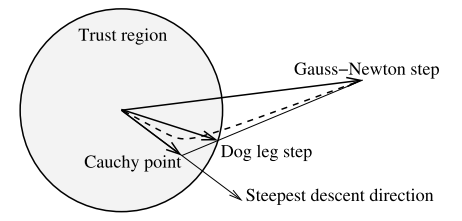
\includegraphics[width=0.75\textwidth]{images/dogleg}
  \caption{Dog leg approximation of the curved optimal trajectory (shown dashed) (Figure taken from \cite{Lourakis2005})}
  \label{fig:dogleg}
\end{figure}

The dog leg step is defined as follows: If the Cauchy point lies outside the trust region, the \ac{DL} step is chosen as the truncated Cauchy step, i.e. the intersection of the Cauchy step with the boundary of the trust region. Otherwise, and if the Gauss-Newton step is within the trust region, the \ac{DL} step is taken to be equal to it. Finally, when the Cauchy point is in the trust region and the Gauss-Newton step is outside, the next trial point is computed as the intersection of the boundary of the trust region and the straight line joining the Cauchy point and the Gauss-Newton step, as shown in \autoref{fig:dogleg}. In every case, the dog leg path intersects the boundary of the trust region at most once and the point of intersection can be determined analytically, without search.\\

The advantage of the \ac{DL} algorithm is, that once the Gauss-Newton step has been determined, the \ac{DL} algorithm can solve the subproblem for various values of $\Delta$, without the need to resolve \autoref{eq:dlgn}.

\subsection{\acf{DL} vs. \acf{LM}}
In the previous sections, the disadvantage of the \ac{LM} algorithm and the advantage of the \ac{DL} algorithm were already mentioned. In this section they will be recapitulated shortly and a conclusion will be drawn.\\

When a \ac{LM} step fails, the \ac{LM} algorithm has to resolve the augmented normal equations with an increased damping term. In other words, every update to the damping term requires that the augmented normal equations are solved again. Therefore failed steps entail unproductive effort.\\
Opposite to this, once the Gauss-Newton step has been calculated, the \ac{DL} algorithm can solve the subproblem for various values of $\Delta$ without solving \autoref{eq:dlgn} again.\\
Another fact is, that when the truncated Cauchy step is taken, the \ac{DL} algorithm can avoid solving \autoref{eq:dlgn}, while the \ac{LM} algorithm always needs to solve \autoref{eq:augnormal}, even if it chooses a step smaller than the Cauchy step.\\

Since the \ac{PGO} and the \ac{BA} problem involves many parameters, linear algebra costs dominate the computational overhead associated with every inner iteration of both algorithms (\ac{LM} and \ac{DL}) and therefore reducing the number of times that \autoref{eq:dlgn} needs to be solved is crucial for the overall performance of the minimization process.\\
For the mentioned reasons, the \ac{DL} algorithm is a more promising implementation of the non-linear minimization arising in \ac{PGO} and \ac{BA} in terms of the required computational effort.
